% ============================================================
% Capítulo VII — Reflexión (Parte A: §§199-216)
% Traducción de "Théorie mathématique de la lumière" (1889), cap. VII
% Original: §§199-216, páginas impresas 320-358
% Parte A: reflexión vítrea — teorías de Fresnel, de Neumann y
% Mac-Cullagh, y de Cauchy. Continúa en la Parte B (reflexión
% cristalina y metálica), a partir de "Réflexion cristalline".
% ============================================================
\chapter{Reflexión}
\label{cap:reflexion}

\section{Reflexión vítrea}

\noindent La reflexión vítrea ha dado lugar a tres teorías igualmente
confirmadas por la experiencia: son la de Fresnel, la de Neumann y
Mac-Cullagh, y la de Cauchy.

\subsection{Teoría de Fresnel}
\label{sec:reflexion-fresnel}

\subsubsection{Hipótesis fundamentales}

\noindent\textbf{199. Hipótesis fundamentales.} — Fresnel supone:

$1^\circ$ Que la vibración es perpendicular al plano de polarización.

$2^\circ$ Que la elasticidad $\varepsilon$ del éter es constante y es la
misma en los dos medios. La densidad $\rho$ del éter es, por el contrario,
variable. Como la velocidad de propagación $V$ es igual a
$\sqrt{\varepsilon/\rho}$, debemos admitir, si consideramos $\varepsilon$
como constante, que $\rho$ es proporcional al cuadrado del índice de
refracción.

$3^\circ$ Fresnel considera luego las velocidades de dos moléculas
infinitamente vecinas una de otra y de la superficie de separación, pero
situadas a uno y otro lado de esta superficie; descompone cada una de
estas velocidades en otras dos, una paralela al plano tangente a la
superficie de separación, la otra normal a este plano. Admite que las
componentes tangenciales de las velocidades de las dos moléculas deben ser
las mismas en magnitud y dirección, pero que las componentes normales
pueden ser diferentes.\footnote{\emph{Œuvres complètes}, t.~I, p.~767.}

Esta manera de enunciar la hipótesis de la continuidad puede parecer
arbitraria a muchos espíritus. Creemos que es un error. Las vibraciones
del éter son transversales; hemos mostrado (§45) que se puede explicar
esta transversalidad de muchas maneras, pero hemos insistido sobre todo en
dos de esas explicaciones. Se puede suponer que esta transversalidad es el
resultado de una suerte de ligadura, tal que la resistencia del éter a la
compresión sea infinita. Es así, como lo hemos dicho más arriba, la
hipótesis que Fresnel parece haber adoptado en su teoría de la doble
refracción. Aquí adopta la hipótesis contraria, aquella en que las
ecuaciones del movimiento se escriben:
\[
\rho\frac{d^2\xi}{dt^2}=\varepsilon\left(\Delta\xi-\frac{d\Theta}{dx}\right),
\qquad
\rho\frac{d^2\eta}{dt^2}=\varepsilon\left(\Delta\eta-\frac{d\Theta}{dy}\right),
\qquad
\rho\frac{d^2\zeta}{dt^2}=\varepsilon\left(\Delta\zeta-\frac{d\Theta}{dz}\right),
\]
y donde la resistencia del éter a la compresión es nula. Pero, siendo así,
nada impide admitir que las componentes normales de las velocidades de
nuestras dos moléculas infinitamente vecinas sean diferentes. Imaginemos,
en efecto, que la superficie de separación de los dos medios sea un plano
y consideremos dos planos infinitamente vecinos, paralelos al plano de
separación, pero situados de una y otra parte de este plano. Pensemos en
las moléculas de éter situadas en estos dos planos; si las componentes
normales de sus velocidades no son las mismas, la distancia de estos dos
planos variará de manera periódica y resultarán de ello compresiones y
dilataciones alternativas del éter comprendido entre estos dos planos.
Pero, siendo nula la resistencia del éter a la compresión, estas
alternativas podrán producirse sin aportar al movimiento ninguna
perturbación.

$4^\circ$ Finalmente, Fresnel se apoya en el principio de las fuerzas
vivas.

\subsubsection{Aplicación de los principios anteriores}

\noindent\textbf{200. Aplicación de los principios anteriores.} —
Supondremos que la superficie de separación de los dos medios es un plano;
que las ondas incidente, reflejada y refractada son planas. Supondremos
además que el rayo incidente, y por consiguiente los rayos reflejado y
refractado, están enteramente polarizados. Las leyes de la reflexión de la
luz natural se deducen en efecto fácilmente de las de la luz polarizada,
si se considera un rayo natural como la superposición de dos rayos de
igual intensidad polarizados en ángulo recto.

Tomaremos el plano de separación de los dos medios como plano de las
$xy$. Sean $\xi,\eta,\zeta$ las tres componentes del desplazamiento de una
molécula cualquiera; $\xi_1,\eta_1,\zeta_1$ las componentes del
desplazamiento debido a la luz incidente; $\xi_2,\eta_2,\zeta_2$ las del
desplazamiento debido a la luz reflejada; $\xi_3,\eta_3,\zeta_3$ las del
desplazamiento debido a la luz refractada. Tendremos entonces, en el
primer medio,
\[
\xi=\xi_1+\xi_2,\qquad \eta=\eta_1+\eta_2,\qquad \zeta=\zeta_1+\zeta_2,
\]
y en el segundo medio:
\[
\xi=\xi_3,\qquad \eta=\eta_3,\qquad \zeta=\zeta_3.
\]
Según la tercera hipótesis de Fresnel, $\xi$ y $\eta$ son funciones
continuas, pero $\zeta$ puede ser discontinua. Se tiene, pues, para
$z=0$,
\begin{equation}
\xi_1+\xi_2=\xi_3,\qquad \eta_1+\eta_2=\eta_3.
\end{equation}

Siendo planas las ondas, tendremos
\[
\xi_1=A_1\cos(P_1+\omega_1),\qquad \eta_1=B_1\cos(P_1+\omega_1'),\qquad
\zeta_1=C_1\cos(P_1+\omega_1'');
\]
o bien
\[
P_1=\frac{2\pi}{\lambda_1}(\alpha_1x+\beta_1y+\gamma_1z-Vt);
\]
\[
\xi_2=A_2\cos(P_2+\omega_2),\qquad \eta_2=B_2\cos(P_2+\omega_2'),\qquad
\zeta_2=C_2\cos(P_2+\omega_2'');
\]
o bien
\[
P_2=\frac{2\pi}{\lambda_2}(\alpha_2x+\beta_2y+\gamma_2z-Vt);
\]
\[
\xi_3=A_3\cos(P_3+\omega_3),\qquad \eta_3=B_3\cos(P_3+\omega_3'),\qquad
\zeta_3=C_3\cos(P_3+\omega_3'');
\]
o bien
\[
P_3=\frac{2\pi}{\lambda_3}(\alpha_3x+\beta_3y+\gamma_3z-V't).
\]

Las $A$, las $B$ y las $C$, y las $\omega$, son constantes; $V$ tiene el
mismo valor para el rayo incidente y para el rayo reflejado, pues es la
velocidad de propagación en el primer medio; $V'$ es la velocidad de
propagación en el segundo medio, y se tiene, llamando $n$ al índice de
refracción,
\[
V'=\frac{V}{n}.
\]

Debiendo estar las vibraciones en el plano de la onda, tendremos
\begin{equation}
\alpha_1\xi_1+\beta_1\eta_1+\gamma_1\zeta_1
=\alpha_2\xi_2+\beta_2\eta_2+\gamma_2\zeta_2
=\alpha_3\xi_3+\beta_3\eta_3+\gamma_3\zeta_3=0.
\end{equation}

La primera de las ecuaciones (1), que debe ser verificada para $z=0$, nos
da
\begin{align}
&A_1\cos\!\left[\frac{2\pi}{\lambda_1}(\alpha_1x+\beta_1y-Vt)+\omega_1\right]
+A_2\cos\!\left[\frac{2\pi}{\lambda_2}(\alpha_2x+\beta_2y-Vt)+\omega_2\right]
\notag\\
&\hspace{3cm}=A_3\cos\!\left[\frac{2\pi}{\lambda_3}(\alpha_3x+\beta_3y-V't)+\omega_3\right].
\end{align}

\noindent\textbf{201.} Fresnel introduce aquí una hipótesis nueva; es que
$\omega_1=\omega_2$; esta hipótesis no le es sugerida por puntos de vista
teóricos, sino por la experiencia, que le prueba que, mientras no haya
reflexión total, la luz reflejada permanece polarizada rectilíneamente si
la luz incidente lo está ella misma.

En este caso la ecuación (3) no puede verificarse idénticamente más que si
se tiene
\begin{equation}
\frac{\alpha_1}{\lambda_1}=\frac{\alpha_2}{\lambda_2}=\frac{\alpha_3}{\lambda_3},
\qquad
\frac{\beta_1}{\lambda_1}=\frac{\beta_2}{\lambda_2}=\frac{\beta_3}{\lambda_3},
\qquad
\frac{V}{\lambda_1}=\frac{V}{\lambda_2}=\frac{V'}{\lambda_3},
\end{equation}
\[
\omega_1=\omega_2=\omega_3,
\qquad A_1+A_2=A_3.
\]
La segunda ecuación (1) nos daría de la misma manera
\[
\omega_1'=\omega_2'=\omega_3',\qquad B_1+B_2=B_3.
\]

Las ecuaciones (4) nos dan
\[
\lambda_1=\lambda_2,\qquad \alpha_1=\alpha_2,\qquad \beta_1=\beta_2,
\qquad \lambda_3=\frac{\lambda_1}{n},\qquad \alpha_3=\frac{\alpha_1}{n},
\qquad \beta_3=\frac{\beta_1}{n}.
\]

Supondremos que el plano de incidencia haya sido elegido como plano de
las $xz$; tendremos entonces $\beta_1=0$ y, llamando $i$ al ángulo de
incidencia:
\[
\alpha_1=\sin i,\qquad \gamma_1=\cos i.
\]
Si $\beta_1$ es nulo, deberá serlo también $\beta_2$ y $\beta_3$, en
virtud de las ecuaciones (4). Esto significa que la onda reflejada y la
onda refractada son perpendiculares al plano de las $xz$, o en otros
términos que el rayo reflejado y el rayo refractado están en el plano de
incidencia.

Puesto que $\alpha_1=\alpha_2$, tendremos también
\[
\alpha_2=\sin i
\]
y
\[
\gamma_2=\pm\sqrt{1-\alpha_2^2-\beta_2^2}=\pm\cos i.
\]
Como $\gamma_2$ no puede ser igual a $\gamma_1$ sin que el rayo incidente
y el reflejado se confundan, tendremos
\[
\gamma_2=-\gamma_1=-\cos i.
\]
Esto muestra que el ángulo de reflexión es igual al ángulo de incidencia.

De la misma manera, si $r$ es el ángulo de refracción, tendremos
\[
\alpha_3=\sin r,\qquad \gamma_3=\cos r,
\]
y puesto que $\alpha_1=n\alpha_3$, se llega a la ley conocida de la
refracción
\[
\sin i=n\sin r.
\]

La teoría de Fresnel conduce, pues, muy simplemente a las leyes
elementales de la reflexión y de la refracción.

Por otra parte, las ecuaciones (2) se convierten en
\[
A_1\alpha_1\cos(P_1+\omega_1)+C_1\gamma_1\cos(P_1+\omega_1'')=0,
\]
\[
A_2\alpha_2\cos(P_2+\omega_2)+C_2\gamma_2\cos(P_2+\omega_2'')=0,
\]
\[
A_3\alpha_3\cos(P_3+\omega_3)+C_3\gamma_3\cos(P_3+\omega_3'')=0.
\]
Estas ecuaciones no pueden verificarse idénticamente más que si se tiene
\[
A_1\alpha_1+C_1\gamma_1=A_2\alpha_2+C_2\gamma_2=A_3\alpha_3+C_3\gamma_3=0
\]
\[
\omega_1=\omega_1'',\qquad \omega_2=\omega_2'',\qquad \omega_3=\omega_3''.
\]

Si el rayo incidente está polarizado rectilíneamente, tendremos
$\omega_1=\omega_1'$; de modo que las nueve cantidades $\omega$ serán
iguales; podremos entonces suponer que el origen de los tiempos ha sido
elegido de tal manera que estas nueve cantidades sean nulas. Nos quedarán,
pues, entre las cantidades $A$, $B$ y $C$, las relaciones:
\begin{equation}
A_1+A_2=A_3,\qquad B_1+B_2=B_3,
\end{equation}
\begin{equation}
A_1\alpha_1+C_1\gamma_1=0,\qquad A_2\alpha_1-C_2\gamma_1=0,\qquad
A_3\alpha_3+C_3\gamma_3=0.
\end{equation}

\subsubsection{Aplicación del principio de las fuerzas vivas}

\noindent\textbf{202. Aplicación del principio de las fuerzas vivas.} —
Para poder aplicar el principio de las fuerzas vivas, es necesario suponer
que solo una porción del éter está perturbada; pues si todo el espacio
estuviera iluminado, la fuerza viva total sería infinita y la aplicación
del principio se volvería ilusoria.

Supondremos que, en el origen de los tiempos, el éter perturbado se
encuentra encerrado en un paralelepípedo rectangular $CDEF$
(figura~\ref{fig:cap7-1}) limitado por dos planos paralelos al plano de
incidencia, por dos planos paralelos al plano de la onda incidente y por
dos planos perpendiculares a los cuatro primeros. Supondremos además que
las dimensiones de este paralelepípedo sean muy grandes respecto a una
longitud de onda, de manera que no haya que tener en cuenta los fenómenos
de difracción.

\begin{figure}[h]
\centering
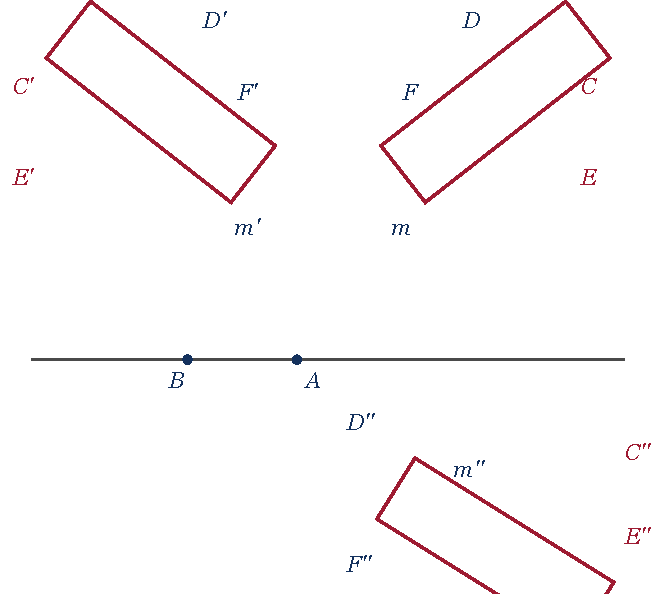
\includegraphics[width=0.85\textwidth]{figuras/pdf/cap07-fig1.pdf}
\caption{El paralelepípedo de éter perturbado $CDEF$ se divide, al cabo
del tiempo $t$, en un paralelepípedo reflejado $C'D'E'F'$ y uno
refractado $C''D''E''F''$.}
\label{fig:cap7-1}
\end{figure}

¿En qué se convertirá la perturbación del éter al cabo de un tiempo $t$?
La perturbación partida de un punto $m$ del paralelepípedo $CDEF$ caminará
primero en la dirección del rayo incidente hasta su encuentro en $\mu$ con
el plano de separación; allí se dividirá en dos partes, una irá de $\mu$ a
$m'$ siguiendo el rayo reflejado, la otra de $\mu$ a $m''$ siguiendo el
rayo refractado. Caminará además con una velocidad $V$ a lo largo de
$m\mu$ y de $\mu m'$ y con una velocidad $V'$ a lo largo de $\mu m''$, de
modo que se deberá tener
\[
\frac{m\mu}{V}+\frac{\mu m'}{V}=\frac{m\mu}{V}+\frac{\mu m''}{V'}=t,
\]
o bien
\begin{equation}
n\cdot\mu m''=\mu m'.
\end{equation}

Así, al tiempo $t$, la luz partida del paralelepípedo $CDEF$ ocupará dos
paralelepípedos: el primero, $C'D'E'F'$, ocupado por la luz reflejada,
tendrá dos caras paralelas al plano de incidencia y dos caras paralelas a
la onda reflejada. El segundo, $C''D''E''F''$, ocupado por la luz
refractada, tendrá dos caras paralelas al plano de incidencia y dos caras
paralelas a la onda refractada. En la figura estos tres paralelepípedos
están representados tomando como plano del dibujo el plano de incidencia.

Sean $q_1,q_2,q_3$ las masas de éter contenidas en estos tres
paralelepípedos. El valor medio de la energía de una masa de éter
perturbada, por ejemplo por la luz incidente, será proporcional, por una
parte, a esta masa, por otra parte a $A_1^2+B_1^2+C_1^2$; el teorema de
las fuerzas vivas se escribirá, pues:
\[
q_1(A_1^2+B_1^2+C_1^2)=q_2(A_2^2+B_2^2+C_2^2)+q_3(A_3^2+B_3^2+C_3^2).
\]

Es claro que $q_1=q_2$; hay que buscar la razón de $q_3$ a $q_1$. Los
volúmenes de nuestros paralelepípedos estarán entre ellos como sus
secciones hechas por el plano de incidencia, es decir, como los
rectángulos $CDEF$, $C''D''E''F''$. Como por otra parte la densidad en el
segundo medio es $n^2$ veces mayor que en el primero, tendremos
\[
\frac{q_3}{q_1}=n^2\,\frac{C''E''}{CE}\cdot\frac{C''D''}{CD}.
\]

Se tiene, en virtud de la ecuación (7):
\[
\frac{C''A}{C'A}=\frac{1}{n},\qquad \frac{E''A}{E'A}=\frac{1}{n},
\]
de donde
\[
C''E''=\frac{1}{n}C'E'=\frac{1}{n}CE.
\]
Por otra parte,
\[
C''D''=AB\cos r,\qquad CD=AB\cos i,
\]
de donde
\[
\frac{q_3}{q_1}=n\,\frac{\cos r}{\cos i}
=\frac{\sin i\cos r}{\sin r\cos i}=\frac{\alpha_1}{\gamma_1}\,\frac{\gamma_3}{\alpha_3}.
\]

El principio de las fuerzas vivas puede entonces escribirse
\[
\frac{\gamma_1}{\alpha_1}(A_1^2+B_1^2+C_1^2-A_2^2-B_2^2-C_2^2)
=\frac{\gamma_3}{\alpha_3}(A_3^2+B_3^2+C_3^2).
\]

Podemos descomponer el rayo incidente en otros dos, uno polarizado en el
plano de incidencia, el otro perpendicularmente a este plano.

Para el primero, $A_1,C_1,A_2,C_2,A_3,C_3$ son nulos.

Para el segundo, $B_1,B_2$ y $B_3$ son nulos.

El principio de las fuerzas vivas debe ser cierto para cada uno de estos
rayos por separado, de modo que la ecuación de las fuerzas vivas se
descompone en dos:
\begin{equation}
\frac{\gamma_1}{\alpha_1}(B_1^2-B_2^2)=\frac{\gamma_3}{\alpha_3}B_3^2,
\end{equation}
\begin{equation}
\frac{\gamma_1}{\alpha_1}(A_1^2-A_2^2+C_1^2-C_2^2)
=\frac{\gamma_3}{\alpha_3}(A_3^2+C_3^2).
\end{equation}

Las ecuaciones (5), (6), (8) y (9) bastan para determinar $A_2,B_2,C_2$ y
$A_3,B_3,C_3$ cuando se conocen $A_1,B_1$ y $C_1$.

\subsubsection{Primeras consecuencias}

\noindent\textbf{203. Primeras consecuencias.} — Si dividimos la ecuación
(8) por la segunda de las ecuaciones (5), resulta:
\begin{equation}
\frac{\gamma_1}{\alpha_1}(B_1-B_2)=\frac{\gamma_3}{\alpha_3}B_3.
\end{equation}

Si en la ecuación (9) reemplazamos $C_1$, $C_2$ y $C_3$ por sus valores
tomados de (6), resulta
\[
\frac{\gamma_1}{\alpha_1}\left(1+\frac{\alpha_1^2}{\gamma_1^2}\right)(A_1^2-A_2^2)
=\frac{\gamma_3}{\alpha_3}\left(1+\frac{\alpha_3^2}{\gamma_3^2}\right)A_3^2,
\]
o dividiendo por la primera ecuación (5),
\[
\frac{\gamma_1}{\alpha_1}\left(1+\frac{\alpha_1^2}{\gamma_1^2}\right)(A_1-A_2)
=\frac{\gamma_3}{\alpha_3}\left(1+\frac{\alpha_3^2}{\gamma_3^2}\right)A_3,
\]
o bien
\begin{equation}
\frac{A_1-A_2}{\alpha_1\gamma_1}=\frac{A_3}{\alpha_3\gamma_3}.
\end{equation}

Las dos ecuaciones (8) y (9) pueden, pues, ser reemplazadas por las
ecuaciones (10) y (11), que tienen la ventaja de ser lineales.

La ecuación (10) puede escribirse (si se recuerda que
$\gamma_2=-\gamma_1$, $\lambda_2=\lambda_1$, $\alpha_1/\lambda_1=\alpha_3/\lambda_3$):
\begin{equation}
\frac{B_1\gamma_1}{\lambda_1}+\frac{B_2\gamma_2}{\lambda_2}
=\frac{B_3\gamma_3}{\lambda_3}.
\end{equation}

De la misma manera la ecuación (11) puede escribirse
\[
A_1\left(\frac{\gamma_1}{\alpha_1}+\frac{\alpha_1}{\gamma_1}\right)
+A_2\left(\frac{\gamma_2}{\alpha_2}+\frac{\alpha_2}{\gamma_2}\right)
=A_3\left(\frac{\gamma_3}{\alpha_3}+\frac{\alpha_3}{\gamma_3}\right),
\]
o teniendo en cuenta las ecuaciones (6)
\[
\frac{A_1\gamma_1-C_1\alpha_1}{\alpha_1}
+\frac{A_2\gamma_2-C_2\alpha_2}{\alpha_2}
=\frac{A_3\gamma_3-C_3\alpha_3}{\alpha_3}.
\]

Esta ecuación y la ecuación (12) se escribirán más simétricamente (al
recordar que los $\beta$ son nulos)
\begin{align}
\frac{B_1\gamma_1-C_1\beta_1}{\lambda_1}
+\frac{B_2\gamma_2-C_2\beta_2}{\lambda_2}
&=\frac{B_3\gamma_3-C_3\beta_3}{\lambda_3},\notag\\
\frac{C_1\alpha_1-A_1\gamma_1}{\lambda_1}
+\frac{C_2\alpha_2-A_2\gamma_2}{\lambda_2}
&=\frac{C_3\alpha_3-A_3\gamma_3}{\lambda_3},
\end{align}
a las cuales se puede añadir la siguiente:
\[
\frac{A_1\beta_1-B_1\alpha_1}{\lambda_1}
+\frac{A_2\beta_2-B_2\alpha_2}{\lambda_2}
=\frac{A_3\beta_3-B_3\alpha_3}{\lambda_3},
\]
que se deduce de la segunda ecuación (5) observando que los $\beta$ son
nulos y que $\alpha_1/\lambda_1=\alpha_2/\lambda_2=\alpha_3/\lambda_3$.

Bajo esta forma simétrica es fácil ver cuál es el significado de las
ecuaciones (13). Tenemos, en efecto, recordando que las cantidades que
habíamos llamado $\omega$ son nulas,
\[
\xi_1=A_1\cos P_1,\qquad \zeta_1=C_1\cos P_1;
\]
de donde
\[
\frac{d\xi_1}{dz}=-\frac{2\pi\gamma_1}{\lambda_1}A_1\sin P_1,
\qquad
\frac{d\zeta_1}{dx}=-\frac{2\pi\alpha_1}{\lambda_1}C_1\sin P_1,
\]
de manera que:
\[
\frac{d\xi_1}{dz}-\frac{d\zeta_1}{dx}=2\pi\sin P_1\,\frac{C_1\alpha_1-A_1\gamma_1}{\lambda_1}.
\]
Así, la segunda ecuación (13) puede escribirse:
\[
\frac{d\xi_1}{dz}-\frac{d\zeta_1}{dx}+\frac{d\xi_2}{dz}-\frac{d\zeta_2}{dx}
=\frac{d\xi_3}{dz}-\frac{d\zeta_3}{dx}.
\]
Ella significa que $\dfrac{d\xi}{dz}-\dfrac{d\zeta}{dx}$ es una función
continua. De la misma manera las otras dos ecuaciones (13) significan que
$\dfrac{d\eta}{dx}-\dfrac{d\xi}{dy}$ y $\dfrac{d\zeta}{dy}-\dfrac{d\eta}{dz}$
son funciones continuas. Estas condiciones pueden reemplazar el principio
de las fuerzas vivas.

Digo que $\dfrac{d\zeta}{dz}$ es también una función continua. En efecto,
$\xi$ y $\eta$ son continuas y es fácil ver que lo mismo ocurre con
$\dfrac{d\xi}{dx}$ y $\dfrac{d\eta}{dy}$. Pero, a causa de la
transversalidad de las vibraciones, se debe tener en los dos medios
\[
\Theta=\frac{d\xi}{dx}+\frac{d\eta}{dy}+\frac{d\zeta}{dz}=0.
\]
Luego $\dfrac{d\zeta}{dz}$ es también continua.

Así, en las hipótesis de Fresnel, no solamente $\xi$ y $\eta$, sino además
$\dfrac{d\xi}{dz}-\dfrac{d\zeta}{dx}$, $\dfrac{d\eta}{dx}-\dfrac{d\xi}{dy}$,
$\dfrac{d\zeta}{dy}-\dfrac{d\eta}{dz}$ y $\dfrac{d\zeta}{dz}$ son funciones
continuas.

\subsubsection{Teorema de Mac-Cullagh}

\noindent\textbf{204. Teorema de Mac-Cullagh.} — Multipliquemos la segunda
ecuación (5) por $\gamma_1/\alpha_1$ y añadámosla a (10) de manera que
eliminemos $B_2$; vendrá
\begin{equation}
2B_1\frac{\gamma_1}{\alpha_1}-B_3\left(\frac{\gamma_1}{\alpha_1}+\frac{\gamma_3}{\alpha_3}\right)=0.
\end{equation}

Eliminemos de la misma manera $A_2$ entre la primera ecuación (5) y la
ecuación (11); vendrá:
\[
2A_1\left(\frac{\gamma_1}{\alpha_1}+\frac{\alpha_1}{\gamma_1}\right)
-A_3\left(\frac{\gamma_1}{\alpha_1}+\frac{\alpha_1}{\gamma_1}
+\frac{\gamma_3}{\alpha_3}+\frac{\alpha_3}{\gamma_3}\right)=0,
\]
o bien
\begin{align}
2A_1\frac{\gamma_1}{\alpha_1}-A_3\left(\frac{\gamma_1}{\alpha_1}+\frac{\gamma_3}{\alpha_3}\right)
&=-2A_1\frac{\alpha_1}{\gamma_1}+A_3\left(\frac{\alpha_1}{\gamma_1}+\frac{\alpha_3}{\gamma_3}\right)
\notag\\
&=\frac{\alpha_1}{\gamma_1}\left[2C_1\frac{\gamma_1}{\alpha_1}-C_3\left(\frac{\gamma_3}{\alpha_3}+\frac{\gamma_1}{\alpha_1}\right)\right].
\end{align}

La comparación de las ecuaciones (14) y (15) da
\[
\begin{vmatrix}A_1&B_1&C_1\\A_3&B_3&C_3\\\alpha_1&0&\gamma_1\end{vmatrix}=0,
\qquad\text{o más simétricamente}\qquad
\begin{vmatrix}A_1&B_1&C_1\\A_3&B_3&C_3\\\alpha_1&\beta_1&\gamma_1\end{vmatrix}=0.
\]

Esta ecuación prueba que el rayo incidente, la vibración incidente y la
vibración refractada están en un mismo plano.

En otros términos la vibración incidente es, en dirección únicamente, la
proyección de la vibración refractada sobre la onda incidente.

Se demostraría de la misma manera que la vibración reflejada es, en
dirección, la proyección de la vibración refractada sobre la onda
reflejada.

\begin{enunciado}{Teorema de Mac-Cullagh (teoría de Fresnel)}
El rayo incidente, la vibración incidente y la vibración refractada están
en un mismo plano: la vibración incidente es, en dirección, la proyección
de la vibración refractada sobre la onda incidente; y de la misma manera,
la vibración reflejada es, en dirección, la proyección de la vibración
refractada sobre la onda reflejada.
\end{enunciado}

\subsubsection{Ley de Brewster}

\noindent\textbf{205. Ley de Brewster.} — Supongamos que el rayo reflejado
sea perpendicular al rayo refractado, es decir, que la onda reflejada sea
perpendicular a la onda refractada.

Toda recta situada en el plano de la onda refractada se proyectará sobre
el plano de la onda reflejada según la recta de intersección de estos dos
planos, es decir, según el eje de las $y$.

Cualquiera que sea, pues, la dirección de la vibración refractada, y por
consiguiente también la dirección de la vibración incidente, la vibración
reflejada será paralela al eje de las $y$.

En otros términos, sea cual sea el plano de polarización del rayo
incidente, el rayo reflejado estará enteramente polarizado en el plano de
incidencia. Será entonces también así cuando la luz incidente sea
natural.

\begin{enunciado}{Ley de Brewster}
Cuando el rayo reflejado es perpendicular al rayo refractado, el rayo
reflejado está enteramente polarizado en el plano de incidencia,
cualquiera que sea el estado de polarización —o la ausencia de ella— del
rayo incidente.
\end{enunciado}

\subsubsection{Reflexión total}

\noindent\textbf{206. Reflexión total.} — Si el segundo medio es menos
refringente que el primero, $n$ es menor que $1$; puede entonces ocurrir
que $\alpha_3$ sea mayor que $1$ y que, en consecuencia, $\gamma_3$ sea
imaginario.

El ángulo de refracción es entonces imaginario, la luz no puede
transmitirse al segundo medio y se refleja toda ella; se dice entonces que
hay reflexión total. En este caso las fórmulas de Fresnel se vuelven
ilusorias, pues la razón $A_2/A_1$, por ejemplo, es imaginaria. Hemos
visto que en el caso ordinario Fresnel había introducido la hipótesis de
que los dos rayos incidente y reflejado tenían la misma fase y que
$\omega_1=\omega_2$.

En el caso de la reflexión total sus fórmulas le dan para $A_2/A_1$ un
valor imaginario de la forma
\[
\cos\varphi+i\sin\varphi.
\]

Fresnel admite, por una suerte de intuición feliz, que el módulo de esta
expresión imaginaria, es decir $1$, representa el verdadero valor de la
razón $A_2/A_1$ y que el argumento de esta misma expresión, es decir
$\varphi$, representa la diferencia de fase $\omega_2-\omega_1$ que había
supuesto hasta entonces nula.

Se vio evidentemente conducido a esta hipótesis audaz por dos experiencias
anteriores que le habían probado que, si el rayo incidente está
polarizado rectilíneamente, el rayo reflejado, que por lo demás tiene la
misma intensidad, está polarizado elípticamente.

Sea cual fuere, su audacia fue plenamente justificada por la experiencia.

\subsubsection{Objeciones contra la teoría de Fresnel}

\noindent\textbf{207. Objeciones contra la teoría de Fresnel.} — El
análisis que precede ha sido entre las manos de Fresnel un admirable
instrumento de descubrimiento; es desde este punto de vista que hay que
considerarlo sin buscarle un rigor que no podría tener. Los teóricos le
han hecho cierto número de objeciones más o menos serias que debemos
refutar si queremos establecer la perfecta concordancia de la teoría de
las ondulaciones con la experiencia.

$1^\circ$ La restricción aportada al principio de la continuidad en lo que
respecta a las componentes normales parece bastante arbitraria;

$2^\circ$ La hipótesis de $\omega_1=\omega_2$ que hemos introducido más
arriba no parece justificada a primera vista por ninguna razón teórica;

$3^\circ$ La fórmula de la reflexión total, confirmada por la experiencia,
parece debida más bien a un feliz azar que a un razonamiento riguroso;

$4^\circ$ Si la elasticidad del éter es constante, su densidad debe ser
proporcional al cuadrado del índice de refracción, pero como este índice
depende de la longitud de onda, esta fórmula conduce, para la densidad del
éter, a valores diferentes según el color de la luz que se considere;

$5^\circ$ Finalmente la teoría anterior no parece, por una razón análoga,
susceptible de extenderse a los medios cristalizados, puesto que el índice
de refracción no es una constante. Si, pues, la densidad se considera como
una constante, no podría ser proporcional al cuadrado de ese índice.

\subsubsection{Refutación de estas objeciones}

\noindent\textbf{208. Refutación de estas objeciones.} — Vamos a buscar
una exposición distinta de la teoría de Fresnel, sin apartarnos del
pensamiento de su autor, pero poniéndonos al abrigo de estas objeciones.

Escribiremos las ecuaciones del movimiento bajo la forma
\[
\rho\frac{d^2\xi}{dt^2}=\varepsilon\left(\Delta\xi-\frac{d\Theta}{dx}\right),
\qquad
\rho\frac{d^2\eta}{dt^2}=\varepsilon\left(\Delta\eta-\frac{d\Theta}{dy}\right),
\qquad
\rho\frac{d^2\zeta}{dt^2}=\varepsilon\left(\Delta\zeta-\frac{d\Theta}{dz}\right).
\]

Consideraremos $\varepsilon$ como constante y $\rho$ como variable;
podremos entonces elegir las unidades de manera que $\varepsilon=1$.
Imaginaremos luego que el espacio se reparte en tres regiones; una
ocupada por el primer medio, y donde $\rho$ podrá considerarse como
constante; otra ocupada por el segundo medio y donde $\rho$ tendrá un
valor constante diferente del de la primera; finalmente entre estas dos
regiones se extenderá una tercera región intermedia, que llamaremos
\emph{capa de paso}, y donde $\rho$ variará muy rápidamente desde su
primer valor constante hasta el segundo. El espesor de esta capa de paso
será finito, pero muy pequeño respecto a una longitud de onda.

Si la superficie de separación es el plano de las $xy$, la capa de paso
estará limitada por dos planos extremadamente vecinos, $z=0$, $z=h$,
paralelos al plano de separación.

Entonces la densidad $\rho$ es una función de $z$ solamente, que
permanece constante de $z=-\infty$ a $z=0$, varía muy rápidamente de $z=0$
a $z=h$ y toma de nuevo un valor constante diferente del primero, de
$z=h$ a $z=+\infty$.

La existencia de semejante capa de paso parecerá más natural que la
hipótesis de un cambio brusco en la naturaleza del medio; nos libra,
además, de todas las dificultades relativas al principio de la
continuidad.

Esto sentado, busquemos satisfacer las ecuaciones del movimiento haciendo:
\[
\xi=\mathrm{X}e^{i(ax+bt)},\qquad \eta=\mathrm{Y}e^{i(ax+bt)},\qquad
\zeta=\mathrm{Z}e^{i(ax+bt)},
\]
siendo X, Y y Z funciones imaginarias de $z$ solamente. Entonces
$\xi,\eta,\zeta$ serán también funciones imaginarias cuyas partes reales
representarán los verdaderos desplazamientos de las moléculas de éter,
conforme a la convención hecha más arriba. Las ecuaciones del movimiento
se convierten entonces en
\[
-\rho b^2\mathrm{X}=\mathrm{X}''-ia\mathrm{Z}',\qquad
-\rho b^2\mathrm{Y}=-a^2\mathrm{Y}+\mathrm{Y}'',\qquad
-\rho b^2\mathrm{Z}=-a^2\mathrm{Z}-ia\mathrm{X}',
\]
representando por letras acentuadas las derivadas de X, Y, Z respecto de
$z$.

En cada uno de los dos medios la densidad $\rho$ es constante y se
encuentra, para la integral de estas ecuaciones,
\[
\mathrm{X}=\mathrm{A}e^{iz\sqrt{\rho b^2-a^2}}+\mathrm{A}'e^{-iz\sqrt{\rho b^2-a^2}},
\]
\[
\mathrm{Y}=\mathrm{B}e^{iz\sqrt{\rho b^2-a^2}}+\mathrm{B}'e^{-iz\sqrt{\rho b^2-a^2}},
\]
\[
\mathrm{Z}=\mathrm{C}e^{iz\sqrt{\rho b^2-a^2}}+\mathrm{C}'e^{-iz\sqrt{\rho b^2-a^2}}.
\]
Llamemos $c$ al valor de $\sqrt{\rho b^2-a^2}$ en el primer medio y $c'$
al valor de este mismo radical en el segundo medio.

Tendremos entonces, comparando nuestras notaciones con las que hemos
empleado más arriba:\footnote{En la última de estas igualdades el
original imprime $\gamma$ en lugar de $b$; se trata de una errata
evidente, pues $b$ es el coeficiente de $t$ en el exponente $i(ax+bt)$.}
\[
a=\frac{2\pi\alpha_1}{\lambda_1}=\frac{2\pi\alpha_2}{\lambda_2}=\frac{2\pi\alpha_3}{\lambda_3},
\qquad
c=\frac{2\pi\gamma_1}{\lambda_1},\qquad c'=\frac{2\pi\gamma_3}{\lambda_3},
\]
\[
b=-\frac{2\pi V}{\lambda_1}=-\frac{2\pi V'}{\lambda_3}.
\]

La expresión de X que acabamos de hallar se compone de dos términos; en el
primer medio, el término en $e^{icz}$ corresponde al rayo incidente y el
término en $e^{-icz}$ corresponde al rayo reflejado; en el segundo medio
el término en $e^{ic'z}$ corresponderá al rayo refractado; el término en
$e^{-ic'z}$ no corresponderá a nada y su coeficiente deberá ser nulo. En
el primer medio tendremos, pues,
\[
\mathrm{X}=\mathrm{A}e^{icz}+\mathrm{A}'e^{-icz},\qquad
\mathrm{Y}=\mathrm{B}e^{icz}+\mathrm{B}'e^{-icz},\qquad
\mathrm{Z}=\mathrm{C}e^{icz}+\mathrm{C}'e^{-icz},
\]
y en el segundo medio
\[
\mathrm{X}=\mathrm{A}''e^{ic'z},\qquad \mathrm{Y}=\mathrm{B}''e^{ic'z},\qquad
\mathrm{Z}=\mathrm{C}''e^{ic'z}.
\]

Si comparamos nuestras notaciones actuales con las que hemos empleado más
arriba, encontraremos:
\[
P_1=ax+cz+bt,\qquad P_2=ax-cz+bt,\qquad P_3=ax+c'z+bt.
\]
\[
\mathrm{A}=A_1e^{i\omega_1},\qquad \mathrm{B}=B_1e^{i\omega_1'},\qquad
\mathrm{C}=C_1e^{i\omega_1''}
\]
\[
\mathrm{A}'=A_2e^{i\omega_2},\qquad \mathrm{B}'=B_2e^{i\omega_2'},\qquad
\mathrm{C}'=C_2e^{i\omega_2''}
\]
\[
\mathrm{A}''=A_3e^{i\omega_3},\qquad \mathrm{B}''=B_3e^{i\omega_3'},\qquad
\mathrm{C}''=C_3e^{i\omega_3''}
\]

Si ponemos
\[
\frac{d\zeta}{dy}-\frac{d\eta}{dz}=u,\qquad
\frac{d\xi}{dz}-\frac{d\zeta}{dx}=v,\qquad
\frac{d\eta}{dx}-\frac{d\xi}{dy}=w,
\]
las ecuaciones del movimiento se convierten en
\[
\rho\frac{d^2\xi}{dt^2}=\frac{dv}{dz}-\frac{dw}{dy},\qquad
\rho\frac{d^2\eta}{dt^2}=\frac{dw}{dx}-\frac{du}{dz},\qquad
\rho\frac{d^2\zeta}{dt^2}=\frac{du}{dy}-\frac{dv}{dx},
\]
o bien:
\[
\frac{du}{dz}=ia w+\rho b^2\eta,\qquad \frac{dv}{dz}=-\rho b^2\xi.
\]

Estas ecuaciones muestran que las derivadas $\dfrac{du}{dz}$ y
$\dfrac{dv}{dz}$ son finitas; y como la capa de paso es extremadamente
delgada, los valores de $u$ y $v$ a los dos lados de esta capa serán
extremadamente poco diferentes. Luego $u$ y $v$ son funciones continuas y
por consiguiente finitas.

Se tiene
\[
\frac{d\xi}{dz}=v+ia\zeta,\qquad \frac{d\eta}{dz}=-u.
\]

Así las derivadas de $\xi$ y de $\eta$ son finitas y por consiguiente
$\xi$ y $\eta$ son continuas. Como por otra parte se tiene
\[
w=ia\eta,
\]
se ve que $w$ es también continua.

Si se suman las tres ecuaciones del movimiento, después de haberlas
diferenciado respectivamente respecto de $x$, $y$ y $z$, viene:
\[
\frac{d(\rho\xi)}{dx}+\frac{d(\rho\eta)}{dy}+\frac{d(\rho\zeta)}{dz}=0,
\]
lo que nos da aquí,\footnote{El original imprime
$\dfrac{d(\rho\zeta)}{dz}=ia\rho\xi$; puesto que
$\dfrac{d(\rho\xi)}{dx}=ia\rho\xi$ y $\dfrac{d(\rho\eta)}{dy}=0$, el signo
correcto es negativo. La errata no afecta al razonamiento, que solo
utiliza la finitud de esta derivada.}
\[
\frac{d(\rho\zeta)}{dz}=-ia\rho\xi.
\]

Esto prueba en primer lugar que $\rho\zeta$ es una función continua y,
como $\rho$ es discontinuo, $\zeta$ no podrá ser continuo a menos de ser
nulo.

Además, siendo $\xi$ continuo, resulta de ello que
\[
\frac{1}{\rho}\,\frac{d(\rho\zeta)}{dz}
\]
es continuo. Pero en los dos medios $\rho$ es constante, $d\rho=0$, de
manera que esta expresión se reduce a $\dfrac{d\zeta}{dz}$.

Así, mediante el cálculo riguroso que precede, reencontramos los mismos
resultados a los que una intuición feliz había conducido a Fresnel: las
funciones $\xi,\eta,u,v,w$ y $\dfrac{d\zeta}{dz}$ son continuas, mientras
que $\zeta$ es discontinua.

Al escribir estas condiciones, resulta\footnote{El original rotula este
sistema como ecuación (15), número que ya había empleado en el §204; se
conserva aquí la numeración impresa, pues el texto se remite a él dos
veces como «(15)» (al final de este párrafo y en el §209).}
\begin{equation}
\begin{gathered}
\mathrm{A}+\mathrm{A}'=\mathrm{A}'',\qquad \mathrm{B}+\mathrm{B}'=\mathrm{B}'',\\
\mathrm{A}c-\mathrm{C}a-\mathrm{A}'c-\mathrm{C}'a=\mathrm{A}''c'-\mathrm{C}''a,
\qquad \mathrm{B}c-\mathrm{B}'c=\mathrm{B}''c',
\end{gathered}
\tag{\thechapter.15}
\end{equation}
a las que hay que añadir las condiciones de transversalidad:\footnote{Se
corrigen aquí dos erratas de signo del original, que imprime
$\mathrm{A}c-\mathrm{C}a+\mathrm{A}'c-\mathrm{C}'a=\mathrm{A}''c'-\mathrm{C}''a$
y $\mathrm{A}''a-\mathrm{C}''c'=0$. Como el término reflejado contiene el
factor $e^{-icz}$ y el refractado el factor $e^{ic'z}$, la continuidad de
$v=\dfrac{d\xi}{dz}-\dfrac{d\zeta}{dx}$ exige $-\mathrm{A}'c$ (en
concordancia con la segunda ecuación (13), donde $\gamma_2=-\gamma_1$, y
con $\mathrm{B}c-\mathrm{B}'c=\mathrm{B}''c'$), y la condición
$\Theta=0$ en el segundo medio da $\mathrm{A}''a+\mathrm{C}''c'=0$, que
es la relación $A_3\alpha_3+C_3\gamma_3=0$ de las ecuaciones (6).}
\[
\mathrm{A}a+\mathrm{C}c=\mathrm{A}'a-\mathrm{C}'c=\mathrm{A}''a+\mathrm{C}''c'=0.
\]

Las condiciones (15) bastan para la solución completa del problema. No
hemos hecho, pues, intervenir el principio de las fuerzas vivas; este
principio es sin embargo ciertamente aplicable en el caso que nos ocupa;
en efecto, las ecuaciones del movimiento de las que nos hemos servido son
las mismas que hemos obtenido en el primer capítulo suponiendo la
existencia de una función de las fuerzas; lo cual implica el principio de
las fuerzas vivas.

\noindent\textbf{209. Reflexión total.} — La cantidad
$c=\dfrac{2\pi\gamma_1}{\lambda_1}$, que se refiere al rayo incidente, es
siempre real; la cantidad $c'$ es también siempre real si el primer medio
es menos refringente que el segundo. Pero, si $n<1$, la cantidad $c'$ no
es real más que si el ángulo de incidencia es bastante pequeño. Si el
ángulo de incidencia sobrepasa cierto límite, $c'$ se vuelve imaginario y
hay reflexión total.

Mientras $c'$ es real, las ecuaciones (15) nos dan para las razones de las
cantidades A, B, C, etc. valores reales; esto equivale a decir que tienen
todas el mismo argumento, o que todas las cantidades $\omega$ son iguales
entre ellas. Si se supone que el origen de los tiempos ha sido elegido de
tal manera que $\omega_1$ sea nulo, las nueve $\omega$ serán nulas. Así se
encuentra justificada la hipótesis de Fresnel.

No ocurre lo mismo cuando $c'$ es imaginario y hay reflexión total; las
razones de los coeficientes A, B, C, etc.\ se volverán imaginarias. Se
vería que las razones
\[
\frac{\mathrm{A}'}{\mathrm{A}},\qquad \frac{\mathrm{B}'}{\mathrm{B}},
\qquad \frac{\mathrm{C}'}{\mathrm{C}}
\]
tienen por módulo la unidad, lo que prueba que la intensidad del rayo
reflejado es la misma que la del rayo incidente. Los argumentos de estas
razones representan las diferencias de fase del rayo reflejado y del rayo
incidente. Así un análisis riguroso, que el empleo de las exponenciales
imaginarias ha vuelto muy simple, nos conduce al mismo resultado que la
inducción audaz de Fresnel.

¿Cuáles serán entonces los movimientos del éter en el segundo medio?
Encontraremos por ejemplo:
\[
\eta=\text{parte real de }\mathrm{B}''e^{i(ax+bt+c'z)}.
\]
Como $c'$ es imaginario podremos poner
\[
c'=ih,
\]
de donde, suponiendo que el origen de los tiempos haya sido elegido de
manera que el argumento de $\mathrm{B}''$ sea nulo,
\[
\eta=\mathrm{B}''e^{-hz}\cos(ax+bt).
\]

Reconocemos así que cierta cantidad de luz penetra en el segundo medio y
que, si no es observable, es a causa de la presencia del factor $e^{-hz}$
que decrece muy rápidamente cuando $z$ crece. Resulta de ello que la
intensidad de la luz refractada no es sensible más que a una débil
distancia del plano de separación, distancia del mismo orden de magnitud
que una longitud de onda.

Se ha logrado detectar la presencia de esta luz refractada\footnote{Quincke,
\emph{Pogg. Ann.}} mediante el siguiente artificio. Dos prismas de vidrio
están separados por una lámina de aire extremadamente delgada; esta
lámina está comprendida entre dos caras paralelas AB y A'B', perteneciendo
la una al primer prisma, la otra al segundo. Un rayo luminoso atraviesa el
primer prisma y viene a encontrar la cara AB bajo un ángulo de incidencia
superior al ángulo límite; la luz refractada penetra en la lámina de aire
y, si esta lámina es lo bastante delgada para que la luz alcance la cara
A'B' antes de haberse extinguido, penetra en el segundo prisma y se
comporta luego regularmente, de manera que se puede observar la luz
transmitida a través de los dos prismas y la lámina de aire.

Esta experiencia parece haber sido hecha por Fresnel\footnote{Fresnel
(?) citado por Verdet, \emph{Leçons d'optique physique}, t.~II.}; ha sido
repetida más recientemente y completada por el Sr. Quincke. El fenómeno es
enteramente análogo al de los anillos coloreados; pero no se observan
entonces las vivas coloraciones que presentan ordinariamente las láminas
delgadas. Es fácil darse cuenta de por qué; en efecto, en la teoría
ordinaria de los anillos coloreados, se encuentra que la intensidad de los
rayos cuya longitud de onda es $\lambda$ es proporcional a
$\sin\dfrac{al}{\lambda}$, designando $l$ el espesor de la lámina y $a$ un
coeficiente que depende de la dirección del rayo luminoso. Para ciertos
valores de $\lambda$, este seno se anula, lo que hace desaparecer los
rayos de ciertos colores y produce una viva coloración de la luz. Aquí
$a$ es imaginario y los senos ordinarios son reemplazados por senos
hiperbólicos que no pueden anularse salvo si $l=0$. Las vivas coloraciones
no aparecerán, pues.

No insistiremos sobre esta experiencia; nos limitaremos a añadir que los
resultados concuerdan con la teoría de una manera bastante satisfactoria,
pero que subsisten sin embargo ligeras diferencias que parecen explicarse
porque el espesor de la capa de paso no sería del todo despreciable frente
a una longitud de onda.

\subsubsection{Objeción relativa a la dispersión}

\noindent\textbf{210. Objeción relativa a la dispersión.} — Las
consideraciones que preceden nos parecen refutar completamente las tres
primeras objeciones hechas a la teoría de Fresnel. Volveremos sobre la
quinta a propósito de la reflexión cristalina; pero debemos hablar aquí
de la cuarta, que es relativa a la dispersión. Para refutarla, hay que
remitirse a lo que hemos dicho acerca de las teorías de la dispersión.

Tomemos por ejemplo la última de las teorías que hemos expuesto. En esta
teoría se considera la acción mutua de las moléculas de éter y de las
moléculas materiales, y las ecuaciones del movimiento se escriben, llamando
$\xi,\eta,\zeta$ las componentes del desplazamiento de una molécula de
éter, $\xi_1,\eta_1,\zeta_1$ las del desplazamiento de una molécula
material, $\rho$ la densidad del éter, $\rho_1$ la de la materia, M un
coeficiente bastante grande:
\[
\rho\frac{d^2\xi}{dt^2}=\Delta\xi-\frac{d\Theta}{dx}+\mathrm{M}(\xi_1-\xi),
\qquad
\rho_1\frac{d^2\xi_1}{dt^2}=\mathrm{M}(\xi-\xi_1),
\]
\[
\rho\frac{d^2\eta}{dt^2}=\Delta\eta-\frac{d\Theta}{dy}+\mathrm{M}(\eta_1-\eta),
\qquad
\rho_1\frac{d^2\eta_1}{dt^2}=\mathrm{M}(\eta-\eta_1),
\]
\[
\rho\frac{d^2\zeta}{dt^2}=\Delta\zeta-\frac{d\Theta}{dz}+\mathrm{M}(\zeta_1-\zeta),
\qquad
\rho_1\frac{d^2\zeta_1}{dt^2}=\mathrm{M}(\zeta-\zeta_1).
\]
M, $\rho$ y $\rho_1$ deben considerarse como funciones de $z$ que,
constantes en cada uno de los dos medios, varían muy rápidamente en la
capa de paso.

Supongamos que se busque satisfacer estas ecuaciones haciendo
\[
\xi=\mathrm{X}e^{i(ax+bt)},\qquad \xi_1=\mathrm{X}_1e^{i(ax+bt)},
\]
\[
\eta=\mathrm{Y}e^{i(ax+bt)},\qquad \eta_1=\mathrm{Y}_1e^{i(ax+bt)},
\]
\[
\zeta=\mathrm{Z}e^{i(ax+bt)},\qquad \zeta_1=\mathrm{Z}_1e^{i(ax+bt)};
\]
se tiene entonces
\[
\frac{1}{\xi}\frac{d^2\xi}{dt^2}=\frac{1}{\eta}\frac{d^2\eta}{dt^2}
=\frac{1}{\zeta}\frac{d^2\zeta}{dt^2}=\frac{1}{\xi_1}\frac{d^2\xi_1}{dt^2}
=\cdots=-b^2,
\]
de donde
\[
\rho_1b^2\xi_1+\mathrm{M}(\xi-\xi_1)=0,\qquad \xi_1=\frac{\mathrm{M}\xi}{\mathrm{M}-\rho_1b^2}.
\]
Pongamos
\[
\rho'=\rho+\frac{\mathrm{M}\rho_1}{\mathrm{M}-\rho_1b^2};
\]
resultará, reemplazando $\xi_1$ por su valor en la primera de las
ecuaciones del movimiento,
\[
-\rho'b^2\xi=\Delta\xi-\frac{d\Theta}{dx},
\]
y de la misma manera
\[
-\rho'b^2\eta=\Delta\eta-\frac{d\Theta}{dy},\qquad
-\rho'b^2\zeta=\Delta\zeta-\frac{d\Theta}{dz}.
\]

Todo ocurre, pues, como si cada uno de los dos medios fuera homogéneo y
tuviera por densidad $\rho'$. Pero esta densidad ficticia $\rho'$ depende
de $b$, es decir, de la longitud de onda. Todo ocurre, pues, como si la
densidad del éter no fuera la misma para los diferentes colores, y la
cuarta objeción se encuentra descartada.

La teoría de Briot, que explica la dispersión admitiendo que $\rho$ no es
una constante sino una función periódica, permite también refutar sin
dificultad esta objeción. Esto no sería tan fácil si se admitiera la
teoría de Cauchy.

\subsection{Teoría de Neumann y Mac-Cullagh}
\label{sec:reflexion-neumann}

\noindent\textbf{211.} Neumann y Mac Cullagh han
fundado, sobre hipótesis enteramente contrarias a las de Fresnel, una
teoría que sin embargo también está confirmada por la experiencia. En el
estudio de esta teoría, adoptaremos un modo de exposición que difiere
mucho del de sus inventores, pero que hace resaltar mejor la verdadera
razón de este hecho singular.

Sean $\xi,\eta,\zeta$ las proyecciones sobre los tres ejes del
desplazamiento debido a la propagación de una onda plana cualquiera, de
manera que $\xi,\eta,\zeta$ sean las partes reales de
\[
\mathrm{A}e^{iP},\qquad \mathrm{B}e^{iP},\qquad \mathrm{C}e^{iP},
\]
o bien
\[
P=\frac{2\pi}{\lambda}(\alpha x+\beta y+\gamma z-Vt).
\]
Si ponemos
\[
u=\frac{d\zeta}{dy}-\frac{d\eta}{dz},\qquad v=\frac{d\xi}{dz}-\frac{d\zeta}{dx},
\qquad w=\frac{d\eta}{dx}-\frac{d\xi}{dy};
\]
$u,v,w$ serán las partes reales de
\[
\mathrm{A}'e^{iP},\qquad \mathrm{B}'e^{iP},\qquad \mathrm{C}'e^{iP},
\]
o bien
\[
\mathrm{A}'=\frac{2\pi i}{\lambda}(\beta\mathrm{C}-\gamma\mathrm{B}),\qquad
\mathrm{B}'=\frac{2\pi i}{\lambda}(\gamma\mathrm{A}-\alpha\mathrm{C}),\qquad
\mathrm{C}'=\frac{2\pi i}{\lambda}(\alpha\mathrm{B}-\beta\mathrm{A}).
\]

Si consideramos $u,v,w$ como las proyecciones sobre los tres ejes del
desplazamiento debido a la propagación de una segunda onda plana, habrá
entre los dos movimientos vibratorios representados respectivamente por
$\xi,\eta,\zeta$ y por $u,v,w$ las relaciones siguientes:

$1^\circ$ Las dos vibraciones $(\xi,\eta,\zeta)$ y $(u,v,w)$ estarán ambas
en el plano de la onda (que será el mismo para los dos movimientos
vibratorios); pero serán perpendiculares la una a la otra.

$2^\circ$ Hay entre las dos vibraciones una diferencia de fase igual a
$\pi/2$ (a causa del factor $i$ que entra en A', B' y C').

$3^\circ$ La amplitud de la vibración $(u,v,w)$ estará con la de la
vibración $(\xi,\eta,\zeta)$ en la razón $2\pi/\lambda$.

\noindent\textbf{212.} Volvamos ahora a la teoría de Fresnel que acabamos
de exponer; hemos visto que si llamamos
$\xi_1,\eta_1,\zeta_1;\xi_2,\eta_2,\zeta_2;\xi_3,\eta_3,\zeta_3$ las
componentes del desplazamiento debido respectivamente a la luz incidente,
a la luz reflejada y a la luz refractada, consideraciones teóricas
condujeron a Fresnel a establecer entre estas nueve cantidades ciertas
relaciones que la experiencia ha confirmado.

Se pueden formar entonces las cantidades $u_1,v_1,w_1;u_2,v_2,w_2;
u_3,v_3,w_3$ de la manera siguiente:
\[
u_1=\frac{d\zeta_1}{dy}-\frac{d\eta_1}{dz},\quad\ldots
\qquad
u_2=\frac{d\zeta_2}{dy}-\frac{d\eta_2}{dz},\quad\ldots
\]

Supongamos con Neumann y Mac Cullagh que la vibración es paralela al
plano de polarización, perpendicular por consiguiente a la vibración de
Fresnel.

Supongamos al mismo tiempo que las tres componentes de las vibraciones
incidente, reflejada y refractada son respectivamente $u_1,v_1,w_1;
u_2,v_2,w_2;u_3,v_3,w_3$, estando estas cantidades ligadas por las mismas
relaciones que en la teoría de Fresnel.

Vamos a mostrar primero que estas hipótesis no son contradichas por la
experiencia, es decir que los resultados verificables experimentalmente
son los mismos que en la teoría de Fresnel.

En efecto, las vibraciones $(\xi,\eta,\zeta)$ y $(u,v,w)$ son
perpendiculares entre ellas, de donde se sigue que la dirección de las
vibraciones incidente, reflejada y refractada es en la teoría de Neumann
perpendicular a lo que es en la teoría de Fresnel; pero, como suponemos al
mismo tiempo que el plano de polarización es paralelo a la vibración y no
perpendicular como lo imaginaba Fresnel, el plano de polarización, que es
lo único accesible a la experiencia, es el mismo en las dos teorías
opuestas.

Sean $\mathrm{I}_1,\mathrm{I}_2,\mathrm{I}_3$ las intensidades de las
luces incidente, reflejada y refractada en la teoría de Fresnel; sean
$\mathrm{I}_1',\mathrm{I}_2',\mathrm{I}_3'$ las intensidades de estas
mismas luces en la teoría de Neumann. Sean $\lambda_1,\lambda_2,\lambda_3$
las longitudes de onda correspondientes.

Como las intensidades son proporcionales a los cuadrados de las
amplitudes, tendremos
\[
\mathrm{I}_1'=\frac{4\pi^2}{\lambda_1^2}\mathrm{I}_1,\qquad
\mathrm{I}_2'=\frac{4\pi^2}{\lambda_2^2}\mathrm{I}_2,\qquad
\mathrm{I}_3'=\frac{4\pi^2}{\lambda_3^2}\mathrm{I}_3.
\]
Como $\lambda_1=\lambda_2=n\lambda_3$ tendremos
\[
\frac{\mathrm{I}_2'}{\mathrm{I}_1'}=\frac{\mathrm{I}_2}{\mathrm{I}_1},\qquad
\frac{\mathrm{I}_3'}{\mathrm{I}_1'}=n^2\frac{\mathrm{I}_3}{\mathrm{I}_1}.
\]

Así la razón de la intensidad de la luz reflejada a la de la luz incidente
es la misma en las dos teorías, de manera que las experiencias que
determinan esta razón no permiten tampoco decidir entre ellas.

La razón $\mathrm{I}_3'/\mathrm{I}_1'$ es por el contrario diferente de la
razón $\mathrm{I}_3/\mathrm{I}_1$; pero si suponemos por ejemplo que el
primer medio sea el aire y el segundo el vidrio, se podrá observar la
intensidad de la luz incidente, pero no se tendrá ningún medio de observar
en el vidrio la de la luz refractada; habrá que esperar, para que esta
observación sea posible, que esta luz haya salido del vidrio por una
nueva refracción para penetrar de nuevo en el aire. Su intensidad se
habrá vuelto entonces $\mathrm{I}_4$ en la teoría de Fresnel,
$\mathrm{I}_4'$ en la de Neumann y, puesto que la longitud de onda será de
nuevo igual a $\lambda_1$ (longitud de onda en el aire), tendremos:
\[
\mathrm{I}_4'=\frac{4\pi^2}{\lambda_1^2}\mathrm{I}_4,
\]
de modo que vendrá aún
\[
\frac{\mathrm{I}_4'}{\mathrm{I}_1'}=\frac{\mathrm{I}_4}{\mathrm{I}_1}.
\]

De la misma manera las experiencias de interferencia, tales como la de
los tres espejos, no pueden permitir dar la preferencia a una de las dos
teorías. Si dos rayos interfieren de manera que se destruyan es porque los
valores de $\xi,\eta,\zeta$ relativos a estos dos rayos son
respectivamente iguales y de signo contrario. Ocurrirá entonces
evidentemente lo mismo con los valores de
\[
u=\frac{d\zeta}{dy}-\frac{d\eta}{dz},\qquad v=\frac{d\xi}{dz}-\frac{d\zeta}{dx},
\qquad w=\frac{d\eta}{dx}-\frac{d\xi}{dy}.
\]

En resumen las dos teorías son ambas igualmente conformes a la
experiencia.

\subsubsection{Principio de continuidad}

\noindent\textbf{213. Principio de continuidad.} — Hemos visto (§203) que
$u,v,w$ son funciones continuas. Como estas funciones representan en la
nueva teoría las componentes del desplazamiento, vemos que estas tres
componentes son continuas. El principio de continuidad no está, pues, ya
sometido aquí a la misma restricción que en la teoría de Fresnel, donde
las componentes paralelas al plano de separación debían ser continuas
mientras que la componente normal podía ser discontinua.

Esta condición de continuidad se expresa escribiendo que, para $z=0$, se
tiene\footnote{A partir de aquí Poincaré reinicia la numeración de las
ecuaciones dentro de la teoría de Neumann y Mac-Cullagh, como ya ha
ocurrido en capítulos anteriores del libro.}
\setcounter{equation}{0}
\begin{equation}
u_1+u_2=u_3;\qquad v_1+v_2=v_3;\qquad w_1+w_2=w_3.
\end{equation}

\subsubsection{Densidad del éter}

\noindent\textbf{214. Densidad del éter.} — Veamos cuál debe ser, en la
nueva teoría, la densidad del éter. Remitámonos a lo que hemos dicho más
arriba a propósito de la aplicación del principio de las fuerzas vivas
(§202). Este principio debe ser aplicable tanto en la hipótesis de
Neumann como en la de Fresnel. Sean $v_1,v_2,v_3$ los volúmenes de tres
paralelepípedos de éter $CDEF$, $C'D'E'F'$ y $C''D''E''F''$. Sean
$\rho_1$ y $\rho_3$ las densidades del éter admitidas por Fresnel en el
primero y el segundo medio; $\rho_1'$ y $\rho_3'$ lo que deben ser estas
mismas densidades en la nueva teoría; se tendrá según una de las
hipótesis de Fresnel
\[
\rho_3=n^2\rho_1.
\]

El principio de las fuerzas vivas se escribirá en la teoría de Fresnel
\begin{equation}
\rho_1(v_1\mathrm{I}_1-v_2\mathrm{I}_2)=\rho_3v_3\mathrm{I}_3,
\end{equation}
y en la de Neumann
\begin{equation}
\rho_1'(v_1\mathrm{I}_1'-v_2\mathrm{I}_2')=\rho_3'v_3\mathrm{I}_3'.
\end{equation}

La ecuación (2) da
\[
v_1\mathrm{I}_1-v_2\mathrm{I}_2=n^2v_3\mathrm{I}_3
\]
de donde
\[
v_1\mathrm{I}_1'-v_2\mathrm{I}_2'=v_3\mathrm{I}_3',
\]
o bien, comparando con (3):
\[
\rho_3'=\rho_1'.
\]

Así en la teoría de Neumann, la densidad del éter debe considerarse como
constante y su elasticidad como la única variable.

En resumen las hipótesis que hemos hecho equivalen a las siguientes, que
son las enunciadas por Neumann y Mac Cullagh:

$1^\circ$ La vibración es paralela al plano de
polarización;\footnote{El original imprime aquí «perpendiculaire», errata
evidente: toda la teoría de Neumann y Mac-Cullagh descansa en la hipótesis
contraria a la de Fresnel (§212), y el propio Poincaré la enuncia como
«La vibration est parallèle au plan de polarisation» en el §217.}

$2^\circ$ La densidad del éter es constante;

$3^\circ$ Las tres componentes del desplazamiento son funciones
continuas.

\subsubsection{Teorema de Mac-Cullagh}

\noindent\textbf{215. Teorema de Mac-Cullagh.} — Sea $O$
(figura~\ref{fig:cap7-2}) un punto del plano de separación; tracemos por
este punto tres rectas $OI$, $OR'$ y $OR$ cuyas proyecciones sobre los
tres ejes sean respectivamente $u_1,v_1,w_1;u_2,v_2,w_2;u_3,v_3,w_3$. Estas
tres rectas representarán, en magnitud y dirección, en la teoría de
Neumann, las vibraciones incidente, reflejada y refractada. Según las
ecuaciones (1), $OR$ es la suma geométrica de $OI$ y $OR'$, es decir, la
diagonal del paralelogramo construido sobre $OI$ y $OR'$. Las tres rectas
$OI$, $OR$ y $OR'$ están, pues, en un mismo plano.

\begin{figure}[h]
\centering
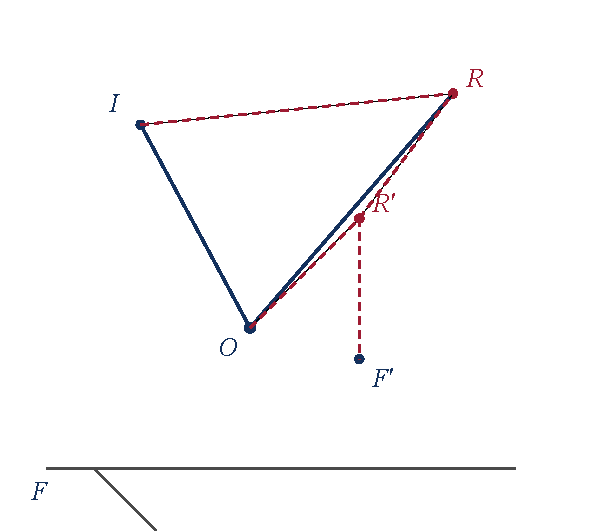
\includegraphics[width=0.75\textwidth]{figuras/pdf/cap07-fig2.pdf}
\caption{Construcción del teorema de Mac-Cullagh: la vibración refractada
$OR$ es la diagonal del paralelogramo construido sobre la vibración
incidente $OI$ y la vibración reflejada $OR'$.}
\label{fig:cap7-2}
\end{figure}

Busquemos determinar este plano. Sean $OF$ y $OF'$ las direcciones de las
vibraciones incidente y refractada en la teoría de Fresnel. El plano
$IOF$ es el de la onda incidente, el plano $ROF'$ el de la onda
refractada.\footnote{El original imprime aquí «le plan R'OF'» y, unas
líneas más abajo, «l'angle IFO»; según la asignación de letras hecha al
comienzo de este párrafo ($OR'$ reflejada, $OR$ refractada) y la
construcción que sigue, debe leerse $ROF'$ e $IOF$, respectivamente.}
Según un teorema demostrado más arriba (§204), $OF$ es la
proyección de $OF'$ sobre la onda incidente; los dos planos $IOF$ y
$F'OF$ son, pues, rectangulares; además el ángulo $IOF$ es recto; luego
$OI$ es perpendicular al plano $FOF'$ y por consiguiente a $OF'$; $OF'$
perpendicular a la vez a $OI$ y a $OR'$ es perpendicular al plano $ROI$.
Luego el plano $ROI$ y el plano de la onda refractada son rectangulares.
Luego \emph{el plano de las tres vibraciones $OI$, $OR$ y $OR'$ pasa por
el rayo refractado.}

Esto permite resolver el siguiente problema: conociendo en magnitud y
dirección la vibración incidente $OI$ (en la teoría de Neumann),
construir las vibraciones reflejada y refractada.

Por $OI$ y el rayo refractado hagamos pasar un plano que corte la onda
reflejada según cierta recta $OR'$ y la onda refractada según una recta
$OR$. Por el punto $I$ tracemos una paralela a $OR'$ hasta su encuentro en
$R$ con $OR$, luego por el punto $R$ una paralela a $OI$ hasta su
encuentro en $R'$ con $OR'$. Hemos construido así en magnitud y dirección
las rectas $OR$ y $OR'$.

Si se quiere enunciar el teorema sin hacer intervenir la dirección de la
vibración, hay que decir:

\begin{enunciado}{Teorema de Mac-Cullagh (teoría de Neumann)}
El plano de polarización del rayo refractado corta el plano de
polarización del rayo incidente según una recta perpendicular al rayo
incidente, y el plano de polarización del rayo reflejado según una recta
perpendicular al rayo reflejado.
\end{enunciado}

\subsection{Teoría de Cauchy}
\label{sec:reflexion-cauchy}

\noindent\textbf{216.}\footnote{\emph{Nouveaux
exercices de mathématiques}, \emph{Comptes rendus}, passim 1836 y 1839.
\emph{Œuvres complètes}, primera serie, t.~IV, passim y principalmente
p.~112 y ss., primera serie, t.~V, p.~111.} Cauchy toma por punto de
partida el principio de continuidad, al cual no aporta ninguna
restricción; no solamente $\xi,\eta$ y $\zeta$ deben ser funciones
continuas, sino que lo mismo ocurre con las derivadas
$\dfrac{d\xi}{dz},\dfrac{d\eta}{dz}$ y $\dfrac{d\zeta}{dz}$ (si se toma
como plano de las $xy$ el plano de separación).

Sería imposible satisfacer estas condiciones si no se admitiera que,
junto a las vibraciones transversales susceptibles de ser observadas, se
propagan igualmente vibraciones longitudinales inaccesibles a la
experiencia. No debemos, pues, admitir que la velocidad de propagación de
los rayos longitudinales sea nula; tampoco puede ser real, pues de lo contrario una
porción de la fuerza viva debida a la luz incidente sería absorbida por
estas ondas longitudinales y la experiencia no indica ningún rastro de
semejante pérdida de fuerza viva.

Nos vemos, pues, conducidos a suponer que esta velocidad de propagación
es imaginaria; será por ejemplo $i\varepsilon$ en el primer medio e
$i\varepsilon'$ en el segundo. Por lo demás $\varepsilon$ y $\varepsilon'$
serán muy pequeños. De esta manera los rayos longitudinales serán
evanescentes (§53) y no absorberán fuerza viva.

Sean $\xi_1,\eta_1,\zeta_1$ las componentes del desplazamiento debido a
las vibraciones transversales, $\xi_2,\eta_2,\zeta_2$ las componentes del
desplazamiento debido a las vibraciones longitudinales, tendremos:
\[
\xi=\xi_1+\xi_2,\qquad \eta=\eta_1+\eta_2,\qquad \zeta=\zeta_1+\zeta_2.
\]

Busquemos satisfacer las condiciones poniendo como más arriba (§210)
\[
\xi_1=\mathrm{X}_1e^{i(ax+bt)},\qquad \eta_1=\mathrm{Y}_1e^{i(ax+bt)},
\qquad \zeta_1=\mathrm{Z}_1e^{i(ax+bt)},
\]
\[
\xi_2=\mathrm{X}_2e^{i(ax+bt)},\qquad \eta_2=\mathrm{Y}_2e^{i(ax+bt)},
\qquad \zeta_2=\mathrm{Z}_2e^{i(ax+bt)},
\]
siendo las X, las Y y las Z funciones de $z$ solamente.

Tendremos, en el primer medio, es decir para $z<0$,
\[
\mathrm{X}_2=\mathrm{A}e^{+hz},\qquad \mathrm{Y}_2=\mathrm{B}e^{+hz},
\qquad \mathrm{Z}_2=\mathrm{C}e^{+hz};
\]
y en el segundo medio, es decir para $z>0$,
\[
\mathrm{X}_2=\mathrm{A}'e^{-h'z},\qquad \mathrm{Y}_2=\mathrm{B}'e^{-h'z},
\qquad \mathrm{Z}_2=\mathrm{C}'e^{-h'z}.
\]

Escribamos que la velocidad de propagación en el primer medio es
$i\varepsilon$, vendrá
\[
\frac{b^2}{a^2-h^2}=-\varepsilon^2\qquad\text{o}\qquad h=\sqrt{a^2+\frac{b^2}{\varepsilon^2}}.
\]
Se encuentra de la misma manera
\[
h'=\sqrt{a^2+\frac{b^2}{\varepsilon'^2}}.
\]

Vemos primero que, siendo $\varepsilon$ y $\varepsilon'$ muy pequeños, $h$
y $h'$ serán muy grandes. Por consiguiente los factores $e^{hz}$ (en el
primer medio donde $z<0$) y $e^{-h'z}$ (en el segundo medio donde $z>0$)
serán muy pequeños a menos que el valor absoluto de $z$ no sea muy
pequeño. No habrá, pues, luz longitudinal sensible más que en la vecindad
inmediata del plano de separación, lo que explica por qué es inobservable
y no absorbe fuerza viva.

Escribamos que la vibración $(\xi_2,\eta_2,\zeta_2)$ es longitudinal;
tendremos:\footnote{Poincaré reinicia aquí la numeración de las
ecuaciones dentro de la teoría de Cauchy, pero el original rotula esta
relación directamente como ecuación (2): ni en el §216 ni en las páginas
que lo preceden desde el comienzo de la teoría de Cauchy figura ninguna
ecuación (1) —un salto de numeración semejante al que ya se documentó en
el Capítulo I (ecuación 37 inexistente) y en el Capítulo IV (ecuación 9
inexistente)—. Se conserva la numeración tal como aparece impresa, pues
el texto se remite después a las «condiciones (2)».}
\setcounter{equation}{1}
\begin{equation}
\frac{d\zeta_2}{dy}-\frac{d\eta_2}{dz}=\frac{d\xi_2}{dz}-\frac{d\zeta_2}{dx}
=\frac{d\eta_2}{dx}-\frac{d\xi_2}{dy}=0.
\end{equation}

Esto muestra que $\dfrac{d\zeta_2}{dy}-\dfrac{d\eta_2}{dz}$ es continuo;
lo es también de
$\dfrac{d\zeta}{dy}-\dfrac{d\eta}{dz}$, puesto que, según el principio de
Cauchy, $\xi,\eta,\zeta$ son continuas así como sus derivadas de primer
orden. Luego
$\dfrac{d\zeta_1}{dy}-\dfrac{d\eta_1}{dz}$ es continuo, de la misma manera
que $\dfrac{d\xi_1}{dz}-\dfrac{d\zeta_1}{dx}$,
$\dfrac{d\eta_1}{dx}-\dfrac{d\xi_1}{dy}$. Así, si no consideramos más que la
luz transversal observable, las cantidades que hemos llamado más arriba
$u,v,w$ son continuas como en la teoría de Fresnel.

Las condiciones (2) pueden también escribirse,
\[
\frac{\mathrm{A}}{a}=\frac{\mathrm{C}}{-ih},\qquad
\frac{\mathrm{A}'}{a}=\frac{\mathrm{C}'}{+ih'},\qquad
\mathrm{B}=\mathrm{B}'=0.
\]
Luego $\eta_2=0$ y, como $\eta$ es continuo, $\eta_1$ deberá serlo también
como en la teoría de Fresnel.

Resulta luego, en el primer medio
\[
h^2\frac{d\xi_2}{dx}+a^2\frac{d\zeta_2}{dz}=0,
\]
y en el segundo medio
\[
h'^2\frac{d\xi_2}{dx}+a^2\frac{d\zeta_2}{dz}=0,
\]
o, lo que es lo mismo, en el primer medio
\begin{equation}
b^2\frac{d\xi_2}{dx}+a^2\varepsilon^2\left(\frac{d\xi_2}{dx}+\frac{d\zeta_2}{dz}\right)=0,
\end{equation}
y en el segundo
\begin{equation}
b^2\frac{d\xi_2}{dx}+a^2\varepsilon'^2\left(\frac{d\xi_2}{dx}+\frac{d\zeta_2}{dz}\right)=0.
\end{equation}

Siendo la vibración $(\xi_1,\eta_1,\zeta_1)$ transversal, tendremos en los
dos medios
\[
\frac{d\xi_1}{dx}+\frac{d\zeta_1}{dz}=0 \qquad (\eta_1 \text{ es
independiente de } y);
\]
y como $\dfrac{d\xi}{dx}+\dfrac{d\zeta}{dz}$ es continuo, esto significa
que $\dfrac{d\xi_2}{dx}+\dfrac{d\zeta_2}{dz}$ es igualmente continuo.

Si llamamos, pues, $\xi_2^0$ y $\zeta_2^0$ los valores de $\xi_2$ y de
$\zeta_2$ en el primer medio, pero infinitamente cerca del plano de
separación, y de la misma manera $\xi_2^1$ y $\zeta_2^1$ los valores de
$\xi_2$ y de $\zeta_2$ en el segundo medio, e infinitamente cerca del
plano de separación, tendremos
\[
\frac{d\xi_2^0}{dx}+\frac{d\zeta_2^0}{dz}=\frac{d\xi_2^1}{dx}+\frac{d\zeta_2^1}{dz};
\]
y las ecuaciones (3) y (4) darán
\begin{equation}
\frac{d\xi_2^1}{dx}-\frac{d\xi_2^0}{dx}
=\frac{a^2}{b^2}(\varepsilon^2-\varepsilon'^2)\left(\frac{d\xi_2^0}{dx}+\frac{d\zeta_2^0}{dz}\right).
\end{equation}

Si la velocidad de propagación de las vibraciones longitudinales fuera la
misma en todos los medios, se tendría $\varepsilon=\varepsilon'$; el
segundo miembro de la igualdad (5) sería nulo y $\dfrac{d\xi_2}{dx}$ sería
continuo.

Resultaría de ello que $\dfrac{d\xi_1}{dx}$ y por consiguiente $\xi_1$
serían funciones continuas y habría concordancia completa con la teoría
de Fresnel.

Pero es más natural suponer $\varepsilon\gtrless\varepsilon'$; en este
caso, como $\varepsilon$ y $\varepsilon'$ son ambos muy pequeños, el
segundo miembro de (5) no es ya nulo sino solamente muy pequeño y la
concordancia con la teoría de Fresnel no es ya más que aproximativa. En
particular el rayo reflejado debería presentar rastros de polarización
elíptica.

La teoría de Cauchy pareció por un instante recibir una confirmación
brillante cuando las experiencias de Jamin revelaron la existencia de
estos rastros de polarización elíptica que el geómetra francés había
previsto. Pero nuevas experiencias del mismo físico cesaron de concordar
con las previsiones de Cauchy.

Sean $i\varepsilon,i\varepsilon',i\varepsilon''$ las velocidades de la luz
longitudinal en el aire, en el agua y en el vidrio; las observaciones de
Jamin sobre la refracción del aire en el vidrio deberían dar la razón
$\varepsilon/\varepsilon''$; de la misma manera observando la refracción
del aire en el agua, luego del agua en el vidrio, se deberían encontrar
las razones $\varepsilon/\varepsilon'$ y $\varepsilon'/\varepsilon''$.

El primer cociente debería ser igual al producto de los otros dos; no es
nada de eso.

Por eso la teoría de Cauchy está hoy abandonada, y se prefiere explicar
los fenómenos observados por Jamin admitiendo que el espesor de la capa
de paso (§208) no es despreciable frente a una longitud de onda.

\section{Reflexión cristalina}
\label{sec:reflexion-cristalina}

Hay dos teorías principales de la reflexión cristalina; la primera es una
extensión de la teoría de Neumann y Mac-Cullagh; la segunda es la de
M.~Sarrau, que puede considerarse como una generalización de las teorías
de Cauchy y de Fresnel.

\subsection{Teoría de Mac-Cullagh}
\label{sec:reflexion-mac-cullagh}

\subsubsection{Hipótesis fundamentales}

\noindent\textbf{217. Hipótesis fundamentales.}\footnote{Mac-Cullagh,
\emph{Transactions} de la Academia Real de Irlanda, vol.~XVIII;
\emph{Journal de Liouville}, primera serie, t.~VII, p.~217. Neumann,
\emph{Journal de Liouville}, primera serie, t.~VII, p.~369, traducción
de una memoria leída en la Academia de Berlín el 7 de diciembre de
1835.} — Mac-Cullagh y Neumann
admiten las mismas hipótesis que en el caso de la reflexión vítrea:

$1^\circ$ La vibración es paralela al plano de polarización;

$2^\circ$ La elasticidad del éter es variable y su densidad constante;

$3^\circ$ El principio de las fuerzas vivas es aplicable;

$4^\circ$ Las tres componentes del desplazamiento $\xi,\eta$ y $\zeta$ son
funciones continuas.

\subsubsection{Ecuaciones del movimiento luminoso}

\noindent\textbf{218. Ecuaciones del movimiento luminoso.} — Recordemos
primero cuáles son las ecuaciones de la doble refracción referidas a ejes
cualesquiera (§179).

Sean X, Y, Z las tres componentes de la vibración de M.~Sarrau; $\xi,\eta,\zeta$
las de la vibración de Neumann, $u,v,w$ las de la vibración de Fresnel;
vendrá:
\[
\xi=\frac{d\mathrm{Z}}{dy}-\frac{d\mathrm{Y}}{dz},\qquad
u=\frac{d\zeta}{dy}-\frac{d\eta}{dz},\qquad
\frac{d^2\mathrm{X}}{dt^2}=\frac{dW_2}{du},
\]
\[
\eta=\frac{d\mathrm{X}}{dz}-\frac{d\mathrm{Z}}{dx},\qquad
v=\frac{d\xi}{dz}-\frac{d\zeta}{dx},\qquad
\frac{d^2\mathrm{Y}}{dt^2}=\frac{dW_2}{dv},
\]
\[
\zeta=\frac{d\mathrm{Y}}{dx}-\frac{d\mathrm{X}}{dy},\qquad
w=\frac{d\eta}{dx}-\frac{d\xi}{dy},\qquad
\frac{d^2\mathrm{Z}}{dt^2}=\frac{dW_2}{dw},
\]
\[
2W_2=au^2+bv^2+cw^2+2evw+2fuw+2guv.
\]
Si se observa que, teniendo en cuenta las expresiones de $u$ y de $v$, se
tiene
\[
\frac{dW_2}{du}=\frac{dW_2}{d\zeta_y'}=-\frac{dW_2}{d\eta_z'},\qquad
\frac{dW_2}{d\xi_x'}=\frac{dW_2}{d\eta_y'}=\frac{dW_2}{d\zeta_z'}=0,\quad\text{etc.,}
\]
vendrá
\[
\frac{d^2\xi}{dt^2}=\frac{d}{dy}\frac{d^2\mathrm{Z}}{dt^2}
-\frac{d}{dz}\frac{d^2\mathrm{Y}}{dt^2}
=-\frac{d}{dy}\frac{dW_2}{d\xi_y'}-\frac{d}{dz}\frac{dW_2}{d\xi_z'},
\]
o
\footnote{A partir de aquí Poincaré reinicia la numeración de las
ecuaciones dentro de la teoría de Mac-Cullagh para la reflexión
cristalina, como ya ha ocurrido varias veces en capítulos anteriores del
libro.}
\setcounter{equation}{0}
\begin{equation}
\frac{d^2\xi}{dt^2}=-\frac{d}{dx}\frac{dW_2}{d\xi_x'}
-\frac{d}{dy}\frac{dW_2}{d\xi_y'}-\frac{d}{dz}\frac{dW_2}{d\xi_z'},
\end{equation}
de donde se deducirían por simetría dos ecuaciones análogas para
$d^2\eta/dt^2$ y $d^2\zeta/dt^2$.

Dicho esto, retomemos la hipótesis de la capa de paso que expusimos más
arriba (§208) y mostremos que esta hipótesis es equivalente a la de
Neumann.

En la teoría de la doble refracción se consideran los coeficientes de
$W_2$ como constantes. Pero aquí no tenemos ya que ver con un medio
homogéneo. Debemos, pues, considerar estos coeficientes $a,b,c,e,f,g$
como variables.

Consideraremos siempre dos
medios separados por una capa de paso extremadamente delgada; esta capa de
paso estará limitada por dos planos paralelos, a saber, por el plano de
las $xy$ y por un plano infinitamente vecino. En cada uno de los dos
medios los coeficientes de $W_2$ conservarán valores constantes; en la
capa de paso, por el contrario, variarán muy rápidamente. Observemos
además que, si uno de los planos que limitan la capa de paso se toma
como plano de las $xy$, estos coeficientes serán funciones de $z$
solamente.

Se tendrá entonces, por ejemplo:
\[
\frac{dW_2}{d\xi_z'}=gu+bv+ew,
\]
y
\[
\frac{d}{dz}\frac{dW_2}{d\xi_z'}=g\frac{du}{dz}+b\frac{dv}{dz}+e\frac{dw}{dz}
+u\frac{dg}{dz}+v\frac{db}{dz}+w\frac{de}{dz}.
\]
Digo ahora que las ecuaciones que acabo de escribir equivalen a las
hipótesis de Neumann y Mac-Cullagh.

\subsubsection{Densidad del éter}

\noindent\textbf{219. Densidad del éter.} — En primer lugar, ellas conllevan el principio de las fuerzas vivas y la
constancia de la densidad del éter. En efecto, hemos visto en el
capítulo~I que, si $\rho$ es la densidad del éter y si
$\int W_2\,d\tau$ representa la función de fuerzas, la ecuación del
movimiento se escribe
\begin{equation}
\rho\frac{d^2\xi}{dt^2}=-\frac{d}{dx}\frac{dW_2}{d\xi_x'}
-\frac{d}{dy}\frac{dW_2}{d\xi_y'}-\frac{d}{dz}\frac{dW_2}{d\xi_z'}.
\end{equation}
Esta ecuación se vuelve idéntica a la ecuación (1) si en ella se hace
$\rho=1$.

La existencia de una función de fuerzas conlleva el principio de las
fuerzas vivas. Se está obligado, por lo demás, para identificar las
ecuaciones (1) y (2), a suponer $\rho=1$, es decir, a considerar la
densidad del éter como constante, lo cual es precisamente la hipótesis de
Neumann.

\subsubsection{Principio de continuidad}

\noindent\textbf{220. Principio de continuidad.} — En segundo lugar, las
ecuaciones del movimiento tal como acabamos de escribirlas conllevan la
continuidad de $\xi,\eta,\zeta$, que constituye la segunda hipótesis de
Neumann.

En efecto, supongamos que se busca satisfacer las ecuaciones del
movimiento haciendo, como lo hemos hecho muchas veces en la teoría de la
reflexión vítrea,
\[
\mathrm{X}=\mathrm{X}_1e^{i(\alpha x+\beta t)},\qquad
\xi=\xi_1e^{i(\alpha x+\beta t)},\qquad
u=u_1e^{i(\alpha x+\beta t)},
\]
\[
\mathrm{Y}=\mathrm{Y}_1e^{i(\alpha x+\beta t)},\qquad
\eta=\eta_1e^{i(\alpha x+\beta t)},\qquad
v=v_1e^{i(\alpha x+\beta t)},
\]
\[
\mathrm{Z}=\mathrm{Z}_1e^{i(\alpha x+\beta t)},\qquad
\zeta=\zeta_1e^{i(\alpha x+\beta t)},\qquad
w=w_1e^{i(\alpha x+\beta t)},
\]
siendo $\mathrm{X}_1,\mathrm{Y}_1,\mathrm{Z}_1,\xi_1,\eta_1,\zeta_1,u_1,v_1,w_1$
funciones de $z$ solamente. Las ecuaciones del movimiento darán:
\[
\frac{d\mathrm{Y}}{dz}=-\xi,\qquad \frac{d\mathrm{X}}{dz}=\eta+i\alpha\mathrm{Z},
\]
\[
\frac{d\eta}{dz}=-u,\qquad \frac{d\xi}{dz}=v+i\alpha\zeta,
\]
\[
\zeta=i\alpha\mathrm{Y},\qquad w=i\alpha\eta.
\]
Estas ecuaciones muestran:

$1^\circ$ Que las derivadas de $\xi,\eta,\mathrm{X}$ y $\mathrm{Y}$ son
finitas y que estas cuatro cantidades son, por consiguiente, continuas;

$2^\circ$ Que $\zeta$ y $w$ son iguales a $\mathrm{Y}$ y a $\eta$, salvo
el factor constante $i\alpha$. Luego $\zeta$ y $w$ son continuos como lo
son $\mathrm{Y}$ y $\eta$ mismos.

Así pues:

$1^\circ$ Las tres componentes $\xi,\eta,\zeta$ de la vibración de Neumann
son continuas;

$2^\circ$ Las dos componentes de la vibración de M.~Sarrau paralelas al
plano de separación, es decir, X e Y, son también continuas.

\subsubsection{Verificaciones experimentales}

\noindent\textbf{221. Verificaciones experimentales.} — Escribiendo que
X, Y, $\xi,\eta$ y $\zeta$ son funciones continuas, se tiene un número
suficiente de ecuaciones para determinar en magnitud y dirección las
vibraciones reflejada y refractada, cuando se conoce la vibración
incidente. No creemos útil, sin embargo, formar aquí estas ecuaciones
lineales y resolverlas efectivamente; no hay en ello más que un cálculo
algebraico bastante largo pero que no presenta ninguna dificultad. Nos
limitaremos a decir que las predicciones de la teoría han sido
confirmadas por la experiencia.

En todas las experiencias que se han hecho, el primer medio era
monorrefringente y el segundo cristalino, y en los desarrollos que
siguen supondremos siempre que es así. Una de las dificultades
principales proviene de que todas las sustancias conocidas son bastante
poco birrefringentes; resulta de ello que el plano de polarización
difiere poco en general de lo que sería con una sustancia isótropa. Se
ha sorteado esta dificultad tomando como primer medio un líquido cuyo
índice de refracción difiere poco del índice medio del cristal. En estas
condiciones se pueden observar desviaciones muy considerables del plano
de polarización. Las desviaciones observadas parecen concordar
suficientemente con las desviaciones calculadas.

Parece, sin embargo, que ciertos cristales presentan anomalías. Así el
diamante, que es del sistema cúbico y debería por consiguiente
comportarse como un cuerpo isótropo, da lugar a una polarización
elíptica muy intensa.

\subsubsection{Refracción uniradial}

\noindent\textbf{222. Refracción uniradial.} — Si un rayo incidente cae
sobre un cristal, se descompone en un rayo reflejado y dos rayos
refractados; estos dos últimos están enteramente polarizados. Supongamos
ahora que el rayo incidente haya sido polarizado por su paso a través de
un nicol; cuando se haga girar este nicol, las intensidades de los dos
rayos refractados variarán; en una de las posiciones del nicol, uno de
los rayos refractados desaparece; en otra posición, es el otro rayo el
que se extingue. Se dice entonces que hay \emph{refracción uniradial}.
Las direcciones de la vibración incidente que corresponden a esta
extinción de uno de los dos rayos refractados se llaman las dos
\emph{direcciones uniradiales}.

\subsubsection{Teorema de Mac-Cullagh}

\noindent\textbf{223. Teorema de Mac-Cullagh.} — El teorema de Mac-Cullagh
(§215) admite una generalización notable por su elegancia,\footnote{Mac-Cullagh,
\emph{Journal de Liouville}, primera serie, t.~VII, 1842.} que
enunciaremos sin demostración.

Hace falta primero dar la definición del plano polar de una de las
vibraciones refractadas. Consideremos uno de los dos rayos refractados;
por un punto $O$ cualquiera tracemos una paralela $ON$ a la vibración de
Neumann y una paralela $OM$ al rayo. Construyamos la superficie de onda
que tiene por centro el punto $O$ y que viene a cortar en $M$ al rayo
luminoso $OM$. En este punto $M$ tracemos el plano tangente a la
superficie de onda y bajemos del punto $M$ una perpendicular $OP$ sobre
este plano tangente; llamaremos $R$ el camino que la luz habría recorrido
en el primer medio durante el tiempo que emplea, en el segundo medio, una
perturbación partida del punto $O$ para llegar al punto $M$ o a un punto
cualquiera de la superficie de onda que pasa por $M$.

\begin{figure}[h]
\centering
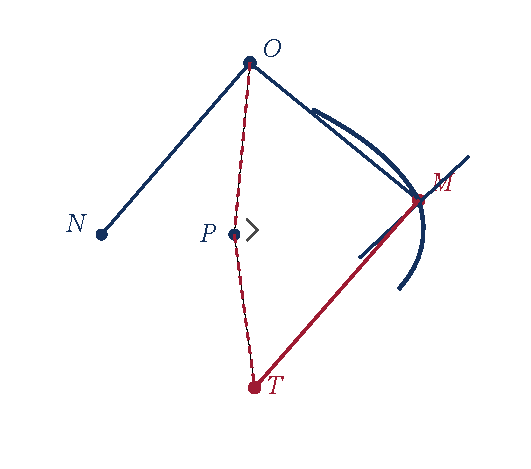
\includegraphics[width=0.45\textwidth]{figuras/pdf/cap07-fig3.pdf}
\caption{Construcción del plano polar de un rayo refractado: el punto
$O$, la paralela $ON$ a la vibración de Neumann, el punto $M$ sobre la superficie de onda, el pie de
la perpendicular $P$ y el punto $T$ tal que $OT=R^2/OP$.}
\label{fig:cap7-3}
\end{figure}

Tomemos luego sobre la prolongación de $OP$ un punto tal que
\[
OT=\frac{R^2}{OP}.
\]
Unamos $MT$; el plano llevado por $ON$ paralelamente a $MT$ se llama el
plano polar del rayo refractado considerado.

Resulta de esta definición que, si se cambia la dirección del plano de
separación haciendo variar al mismo tiempo la dirección del rayo
incidente, pero de tal manera que la del rayo refractado no cambie, el
plano polar tampoco cambiará, con tal de que el índice de refracción del
primer medio permanezca el mismo; la dirección de este plano depende, por
el contrario, del índice de refracción del primer medio.

He aquí ahora en qué consiste el teorema de Mac-Cullagh.

En el caso de la refracción uniradial, se obtendrá el desplazamiento de
un punto cualquiera del primer medio componiendo los desplazamientos
debidos a la vibración incidente y a la vibración reflejada; en cuanto al
desplazamiento de un punto del segundo medio, se reducirá al
desplazamiento debido a la sola vibración refractada que subsiste, puesto
que hemos supuesto el nicol orientado de manera que extinga la segunda
vibración refractada.

Si, pues, construimos en un punto del plano de separación tres rectas que
representen en magnitud y dirección la vibración refractada, la vibración
incidente y la vibración reflejada, la primera será la suma geométrica
de las otras dos. Estas tres rectas están, pues, en un mismo plano.

\begin{enunciado}{Teorema de Mac-Cullagh (reflexión cristalina)}
El análisis de Mac-Cullagh muestra que este plano no es otro que el plano
polar de la vibración refractada.
\end{enunciado}

\noindent\textbf{224.} Propongámonos ahora el siguiente problema:

Conociendo en magnitud y dirección la vibración incidente, construir la
vibración reflejada y las dos vibraciones refractadas.

La construcción de Huygens nos permitirá primero, conociendo el plano de
la onda incidente, construir los planos de la onda reflejada y de las dos
ondas refractadas; conoceremos igualmente el rayo reflejado y los dos
rayos refractados.

Deduciremos de ello las \emph{direcciones} de las dos vibraciones
refractadas $OR'$ y $OR''$; puesto que, en la teoría de Neumann, la
vibración refractada debe estar llevada en el plano de la onda
perpendicularmente al rayo (§215).

Construyamos luego los planos polares de las dos vibraciones refractadas;
estos planos polares cortarán el plano de la onda incidente según las
dos \emph{direcciones uniradiales}.

Sea $OI$ la vibración incidente dada, la descompondremos, por la regla
del paralelogramo, en dos componentes $OI'$ y $OI''$ dirigidas según
estas direcciones uniradiales.

El primer plano polar que pasa por $OR'$ y $OI'$ cortará la onda
reflejada según una recta $OS'$. Terminamos el paralelogramo $OI'R'S'$,
del cual un lado es $OI'$ y del cual el otro lado y la diagonal están
dirigidos según $OS'$ y $OR'$.\footnote{El original nombra estas dos
rectas en el orden «OR' et OS'»; como la vibración refractada es la suma
geométrica de la incidente y la reflejada (§223), la diagonal es $OR'$
y el otro lado $OS'$, tal como se precisa enseguida para el segundo
paralelogramo y como muestra la figura.} Entonces $OR'$ representará, no solamente
en dirección, sino en magnitud, la primera vibración refractada, y $OS'$
representará en magnitud y dirección lo que sería la vibración reflejada
si la vibración incidente se redujera a $OI'$.

\begin{figure}[h]
\centering
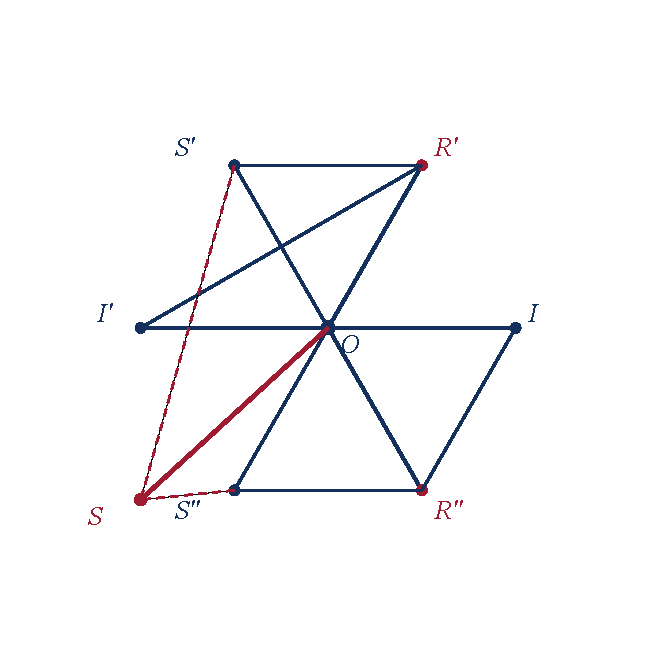
\includegraphics[width=0.6\textwidth]{figuras/pdf/cap07-fig4.pdf}
\caption{Construcción de la vibración reflejada y de las dos vibraciones
refractadas a partir de la incidente $OI$, descompuesta en $OI'$ y
$OI''$ según las direcciones uniradiales.}
\label{fig:cap7-4}
\end{figure}

Se construiría de la misma manera un segundo paralelogramo $OI''R''S''$,
del cual un lado sería $OI''$; del cual la diagonal $OR''$ representaría
en magnitud y dirección la segunda vibración refractada; del cual, en
fin, el segundo lado $OS''$ representaría lo que sería la vibración
reflejada si la vibración incidente se redujera a $OI''$.

No quedará luego más que componer $OS'$ y $OS''$ por la regla del
paralelogramo para tener la vibración reflejada total $OS$.

\subsubsection{Observación}

\noindent\textbf{225. Observación.} — Es fácil darse cuenta, por lo que
precede, de por qué los fenómenos de la reflexión cristalina se apartan
tanto más de los de la reflexión vítrea cuanto más se acerca el índice
del primer medio al índice medio del cristal. En efecto, la separación
entre los dos órdenes de fenómenos será tanto mayor cuanto más se aparte
el plano polar definido más arriba del plano $NOP$; es decir, que el
ángulo $PTM$ será más próximo a $90^{\circ}$. Siendo poco birrefringentes las
sustancias conocidas, el ángulo $POM$ es pequeño y, por consiguiente,
$PM$ es pequeño.

Para que el ángulo $PTM$ no sea pequeño, hace falta que $PT$ sea pequeño.
Ahora bien:
\[
PT=\frac{R^2}{OP}-OP.
\]
Hace falta, pues, que $OP$ sea muy cercano a $R$. Ahora bien, $OP/R$ es la
razón de la velocidad de propagación de la onda refractada a la de la
onda incidente. Estas dos velocidades deben, pues, ser muy cercanas, lo
que exige que los índices medios de los dos medios sean poco diferentes.

\subsection{Teoría de M.~Sarrau}
\label{sec:reflexion-sarrau}

\noindent\textbf{226.}\footnote{\emph{Journal de Liouville}, segunda
serie, t.~XIII.} M.~Sarrau supone:

$1^\circ$ Que la verdadera vibración tiene por componentes las
cantidades que hemos llamado más arriba X, Y y Z;

$2^\circ$ Admite además los principios fundamentales de la teoría de la
reflexión debida a Cauchy, y según los cuales las tres componentes del
desplazamiento serían continuas así como sus derivadas primeras, pero a
condición de tener en cuenta, junto a los rayos transversales
observables, rayos longitudinales evanescentes e inaccesibles a la
experiencia.

Hemos visto más arriba (§216) cuáles eran las consecuencias de los
principios admitidos por Cauchy. Si $\xi_1,\eta_1,\zeta_1$ son las tres
componentes del desplazamiento debido a la luz transversal (tomando el
plano de incidencia por plano de las $xz$ y el plano de separación por
plano de las $xy$), las cantidades
\[
\eta_1,\qquad \frac{d\zeta_1}{dy}-\frac{d\eta_1}{dz},\qquad
\frac{d\xi_1}{dz}-\frac{d\zeta_1}{dx},\qquad
\frac{d\eta_1}{dx}-\frac{d\xi_1}{dy},
\]
son funciones continuas. Si además la velocidad imaginaria de las ondas
longitudinales es la misma en todos los medios, $\xi_1$ es también una
función continua. Aunque por lo demás esta condición no se cumpla,
$\xi_1$ es todavía aproximadamente continua.

Aquí las tres componentes de la verdadera vibración son X, Y y Z; luego
X, Y y
\[
\xi=\frac{d\mathrm{Z}}{dy}-\frac{d\mathrm{Y}}{dz},\qquad
\eta=\frac{d\mathrm{X}}{dz}-\frac{d\mathrm{Z}}{dx},\qquad
\zeta=\frac{d\mathrm{Y}}{dx}-\frac{d\mathrm{X}}{dy}
\]
son funciones continuas. Estos son precisamente los resultados a los que
conducía la teoría de Neumann y Mac-Cullagh; hay, pues, concordancia
perfecta entre las dos teorías.

Importa precisar, en el caso de los medios anisótropos, lo que se debe
entender por rayo longitudinal; las vibraciones longitudinales están
dirigidas no según el rayo, sino normalmente al plano de la onda.

Añadamos que la teoría de M.~Sarrau conduciría al mismo resultado si, en
lugar de tomar por punto de partida las ideas de Cauchy, hubiera supuesto
la existencia de una capa de paso y la variación continua de los
coeficientes del polinomio que hemos llamado $W_2$.

La teoría de la doble refracción de Fresnel (§149) combinada con los
principios de la teoría de la reflexión de Cauchy conduce a resultados
incompatibles con las observaciones.

No ocurre lo mismo si se admite que la verdadera vibración es la de
Fresnel y que existe una capa de paso; los resultados a los que se llega
así no difieren de los que se pueden deducir de las otras dos teorías.

Gracias a la hipótesis de la capa de paso, los fenómenos de la reflexión
cristalina no permiten decidir entre las tres teorías de la doble
refracción; las ecuaciones del §218 conservan en efecto siempre la
misma forma cualquiera que sea la de estas tres teorías que se adopte;
solo difiere la interpretación física. Para M.~Sarrau, son X, Y, Z; para
Neumann, es $\xi,\eta,\zeta$; para Fresnel, son $u,v,w$ los que
representan las componentes de la verdadera vibración. Pero la forma
analítica de las ecuaciones y, por consiguiente, los fenómenos
observables siguen siendo los mismos en estos tres casos.

\section{Reflexión metálica}
\label{sec:reflexion-metalica}

\noindent\textbf{227. Propagación de la luz en un medio absorbente.} —
Los medios opacos, como los metales, deben considerarse, no como
absolutamente impermeables a la luz, puesto que en lámina delgada gozan
de cierta transparencia, sino como dotados de un poder absorbente
considerable.

Veamos cómo se puede concebir la propagación de la luz en un medio
semejante.

Las tres componentes del desplazamiento serán las partes reales de
funciones de la forma
\[
\xi=\mathrm{A}e^{iP},\qquad \eta=\mathrm{B}e^{iP},\qquad
\text{donde}\quad P=\frac{2\pi}{\lambda}(\alpha x+\beta y+\gamma z-Vt).
\]
Pero las cantidades A, B, C, que son proporcionales a la amplitud de la
vibración, deberán decrecer muy rápidamente a medida que el rayo se
propague. La hipótesis más natural será suponer que A, B, C son de la
forma
\[
\mathrm{A}=\mathrm{A}_0e^{-Q},\qquad \mathrm{B}=\mathrm{B}_0e^{-Q},
\qquad \mathrm{C}=\mathrm{C}_0e^{-Q},
\]
o
\[
Q=lx+my+nz;
\]
siendo $\mathrm{A}_0,\mathrm{B}_0,\mathrm{C}_0,l,m$ y $n$ constantes.

Se ve así que, en la propagación de una onda plana en un medio
absorbente, hay que considerar dos planos que desempeñan ambos un papel
importante: el plano de la onda
\[
\alpha x+\beta y+\gamma z=0
\]
y el plano de absorción
\[
lx+my+nz=0.
\]
Las expresiones de $\xi,\eta$ y $\zeta$ pueden también
escribirse\footnote{Con $\mathrm{A}=\mathrm{A}_0e^{-Q}$ se tiene, en
rigor, $\mathrm{A}e^{iP}=\mathrm{A}_0e^{i(P+iQ)}$, es decir, coeficientes
$\frac{2\pi}{\lambda}\alpha+il$, etc., y no $\frac{2\pi}{\lambda}\alpha-il$;
con ese signo la parte imaginaria de $1/V'^2$ resultaría igual a
$+\frac{\lambda}{\pi V^2}(\alpha l+\beta m+\gamma n)$, positiva. Poincaré
adopta en todo lo que sigue (§§227--230) la convención de signo opuesta
para la parte imaginaria ---equivalente a reemplazar las cantidades
imaginarias por sus conjugadas---, de la que dependen la forma
$m(\cos\chi-i\sin\chi)$ del índice y la ecuación (1) del §228. Como el
cambio es global, no altera ninguna conclusión física, y se conserva aquí
el texto del original.}
\[
\xi=\mathrm{A}_0e^{iP'},\qquad \eta=\mathrm{B}_0e^{iP'},\qquad
\zeta=\mathrm{C}_0e^{iP'},
\]
poniendo
\[
P'=\left[\left(\frac{2\pi}{\lambda}\alpha-il\right)x
+\left(\frac{2\pi}{\lambda}\beta-im\right)y
+\left(\frac{2\pi}{\lambda}\gamma-in\right)z-\frac{2\pi V t}{\lambda}\right].
\]
Dicho de otro modo, todo pasa como si el plano de la onda tuviera por
ecuación
\[
P''=\left(\frac{2\pi}{\lambda}\alpha-il\right)x
+\left(\frac{2\pi}{\lambda}\beta-im\right)y
+\left(\frac{2\pi}{\lambda}\gamma-in\right)z=0
\]
y si la velocidad de propagación tuviera por expresión
\[
V'=\dfrac{V}{\sqrt{\left(\alpha-\dfrac{il\lambda}{2\pi}\right)^2
+\left(\beta-\dfrac{im\lambda}{2\pi}\right)^2
+\left(\gamma-\dfrac{in\lambda}{2\pi}\right)^2}}.
\]
Llamaremos al plano $P''=0$ plano imaginario de la onda, y a la velocidad
$V'$, velocidad imaginaria de la onda.

Para que el rayo vaya constantemente debilitándose a medida que se
propaga, es necesario y suficiente que la normal al plano de la onda
llevada en el sentido de la propagación del rayo y la normal al plano de
absorción llevada en el sentido de la extinción formen un ángulo agudo.
Esta condición se escribe:
\[
\alpha l+\beta m+\gamma n>0.
\]
Ahora bien, la parte imaginaria de $1/V'^2$ es igual a
\[
-\frac{\lambda}{\pi V^2}(\alpha l+\beta m+\gamma n).
\]
Esta parte imaginaria\footnote{El original dice «Cette partie réelle»,
errata evidente: la frase anterior acaba de calcular la parte
\emph{imaginaria} de $1/V'^2$, y el párrafo siguiente vuelve a hablar de
«la partie imaginaire du carré de $1/V'$».} debe, pues,
ser negativa.

En resumen, un medio absorbente se comporta como si su índice de
refracción fuera imaginario. Sea
\[
m(\cos\chi-i\sin\chi)
\]
este índice. Como el índice de refracción es proporcional al inverso de
la velocidad, es decir, aquí a $1/V'$, y que la parte imaginaria del
cuadrado de $1/V'$ debe ser negativa, el ángulo $\chi$ deberá estar
comprendido entre $0$ y $\pi/2$.

\noindent\textbf{228.} Dicho esto, propongámonos el siguiente problema:

Un rayo luminoso cae sobre una superficie metálica con una incidencia
igual a $\varphi$; ¿cuál es la dirección del plano imaginario de la
onda, del plano de la onda, del plano de absorción, y el coeficiente de
absorción?

El plano de absorción no puede ser más que el plano de separación de los
dos medios, que tomamos por plano de las $xy$. Tomaremos el plano de
incidencia por plano de las $xz$.

Sea $r'$ el ángulo del plano imaginario de la onda con el plano de las
$xy$, es decir, el ángulo imaginario de refracción. Sea $r$ el ángulo
real de la onda con el plano de las $xy$, es decir, el ángulo real de
refracción.

El plano imaginario de la onda deberá tener por ecuación
\[
x\sin r'+z\cos r'=0,
\]
o\footnote{A partir de aquí Poincaré reinicia la numeración de las
ecuaciones dentro de la sección sobre la reflexión metálica.}
\setcounter{equation}{0}
\begin{equation}
\sin r'=\frac{\sin\varphi}{m}(\cos\chi+i\sin\chi),
\end{equation}
Se tendrá por otra parte
\[
P=\frac{2\pi}{\lambda}(x\sin r+z\cos r-Vt),
\]
y
\[
Q=\varkappa z,
\]
siendo $\varkappa$ el coeficiente de absorción.

La ecuación del plano imaginario de la onda se escribirá entonces
\[
x\frac{2\pi}{\lambda}\sin r+z\left(\frac{2\pi}{\lambda}\cos r-i\varkappa\right)=0,
\]
Se tiene, pues:
\[
\tan r'=\dfrac{\dfrac{2\pi}{\lambda}\sin r}{\dfrac{2\pi}{\lambda}\cos r-i\varkappa}.
\]
De la ecuación (1) se saca fácilmente $\cot r'$ bajo la forma:
\[
\cot r'=\mathrm{A}-i\mathrm{B};
\]
se tiene entonces
\[
\cot r=\mathrm{A},\qquad \varkappa=\frac{2\pi\mathrm{B}\sin r}{\lambda};
\]
lo que determina el ángulo real de refracción y el coeficiente de
absorción.

\subsection{Teoría de Cauchy}
\label{sec:reflexion-metalica-cauchy}

\noindent\textbf{229. Ecuaciones del movimiento luminoso en un medio
absorbente.} — Se han propuesto diversas formas para las ecuaciones del
movimiento en un medio absorbente. Una de las más generales es la de
Voigt,\footnote{\emph{Göttinger Nachrichten}, 1884, p.~137 y ss.} que se
escribe:
\begin{equation}
\rho\frac{d^2\xi}{dt^2}=\Delta\xi+a\xi+b\frac{d\xi}{dt}+c\frac{d\Delta\xi}{dt}
+e\frac{d^2\Delta\xi}{dt^2},
\end{equation}
con otras dos ecuaciones análogas para $\eta$ y $\zeta$, a las cuales hay
que añadir la condición de transversalidad $\Theta=0$.

La teoría electromagnética de la luz ha conducido a Maxwell a una
ecuación de la misma forma, pero donde los coeficientes $a,c$ y $e$ son
nulos.

Estas ecuaciones, u otras análogas, no pueden evidentemente dar cuenta de
la propagación de la luz en los medios poco absorbentes, que producen un
espectro de rayas o de bandas. Cualquiera que sea el número de derivadas
parciales de $\xi$ que en ellas se introduzca, nunca se llegará a dar
cuenta de la prodigiosa variedad de estos espectros. En cambio, estas
ecuaciones parecen dar cuenta bastante bien de los fenómenos ópticos que
presentan los metales.

Busquemos satisfacer la ecuación (2) haciendo
\[
\xi=\mathrm{A}e^{\frac{2i\pi}{V'\tau}(\alpha'x+\beta'y+\gamma'z-V't)}.
\]
La parte real de esta exponencial imaginaria será entonces el verdadero
valor de $\xi$; $\tau$ será el período de la vibración, $V'$ será la
velocidad imaginaria de propagación; $\alpha',\beta',\gamma'$ serán los
cosenos directores del plano imaginario de la onda, de tal manera que se
tendrá
\begin{equation}
\alpha'^2+\beta'^2+\gamma'^2=1.
\end{equation}
Se encuentra entonces, sustituyendo este valor de $\xi$ en (2),
suprimiendo los factores comunes y teniendo en cuenta
(3):\footnote{El original imprime $\dfrac{4\pi^2e}{\tau}$ en el último
término; como $e$ multiplica a una segunda derivada respecto del tiempo,
debe leerse $\dfrac{4\pi^2e}{\tau^2}$. En cuanto a los dos términos
imaginarios, la sustitución directa con el exponente
$\dfrac{2i\pi}{V'\tau}(\ldots-V't)$ los da con signo $-$; el cambio
simultáneo de ambos signos corresponde a la misma convención señalada en
el §227 y no afecta a la conclusión que sigue.}
\begin{equation}
V'^2\left(a+\frac{2i\pi b}{\tau}+\frac{4\pi^2\rho}{\tau^2}\right)
=\frac{4\pi^2}{\tau^2}\left(1+\frac{2i\pi c}{\tau}-\frac{4\pi^2 e}{\tau^2}\right).
\end{equation}
Esta ecuación muestra que la velocidad imaginaria $V'$ depende de $\tau$
y, por consiguiente, de la longitud de onda, pero no depende de la
dirección del plano de la onda.

Por consiguiente, el índice imaginario de refracción $\sin r'/\sin\varphi$
es una constante que depende del color, pero es independiente de la
incidencia. No ocurriría lo mismo con el índice real de refracción
$\sin r/\sin\varphi$.

\noindent\textbf{230. Teoría de Cauchy.}\footnote{\emph{Nouveaux exercices
de mathématiques}, \emph{Journal de Liouville}, primera serie, t.~VII,
p.~338.} — Cauchy supone que las hipótesis que sirven de base a su teoría
de la reflexión vítrea siguen siendo aplicables a la reflexión metálica.

De estas hipótesis resulta, como lo hemos visto, que si el plano de
separación se toma como plano de las $xy$, las funciones
\[
\xi,\qquad \eta,\qquad \frac{d\zeta}{dy}-\frac{d\eta}{dz},\qquad
\frac{d\xi}{dz}-\frac{d\zeta}{dx},\qquad \frac{d\eta}{dx}-\frac{d\xi}{dy}
\]
son continuas.

Acabamos de ver que, en un medio metálico, las ecuaciones del movimiento
son las mismas que si el índice de refracción fuera imaginario. Por otra
parte, en las ideas de Cauchy, las condiciones en el límite son las
mismas que en el caso de la reflexión vítrea. Es, pues, inútil volver a
empezar los cálculos; las fórmulas de la reflexión vítrea deben seguir
siendo aplicables; basta con reemplazar en ellas el índice de refracción
por su valor imaginario.

Sabemos que, en el estudio de la reflexión vítrea, la teoría de Cauchy y
la de Fresnel conducen a los mismos resultados. Fresnel demuestra que la
razón de la vibración reflejada a la vibración incidente es igual a
\[
\frac{\sin(r-\varphi)}{\sin(r+\varphi)}
\]
si la luz está polarizada en el plano de incidencia, y a
\[
\frac{\tan(\varphi-r)}{\tan(\varphi+r)}
\]
si la luz está polarizada perpendicularmente a este plano.

Los ángulos $\varphi$ y $r$ son los ángulos de incidencia y de
refracción. Si se llama N al índice de refracción, estas dos razones son
iguales respectivamente a
\[
\mathrm{A}=\frac{\cos\varphi-\sqrt{\mathrm{N}^2-\sin^2\varphi}}
{\cos\varphi+\sqrt{\mathrm{N}^2-\sin^2\varphi}}
\qquad\text{y}\qquad
\mathrm{A}'=\frac{\mathrm{N}^2\cos\varphi-\sqrt{\mathrm{N}^2-\sin^2\varphi}}
{\mathrm{N}^2\cos\varphi+\sqrt{\mathrm{N}^2-\sin^2\varphi}}.
\]
Estas fórmulas se deducirían sin dificultad de las que hemos dado más
arriba (§203).

Si $\alpha,\beta,\gamma$ son los cosenos directores de la onda reflejada,
$\lambda$ la longitud de onda y V la velocidad de propagación en el
primer medio, el desplazamiento debido a la vibración reflejada será la
parte real de
\[
\mathrm{A}e^{iP}\qquad\text{o}\qquad \mathrm{A}'e^{iP},
\]
o\footnote{El original imprime $\mathrm{P}=\dfrac{2i\pi}{\lambda}(\ldots)$;
el factor $i$ sobra, pues ya figura en el exponente $i\mathrm{P}$ y
$\mathrm{P}$ debe ser real para que el desplazamiento reflejado sea
$\mathrm{A}_0\cos(\mathrm{P}+\psi)$.}
\[
\mathrm{P}=\frac{2\pi}{\lambda}(\alpha x+\beta y+\gamma z-Vt).
\]
Si se pasa a la reflexión metálica, hace falta dar a N un valor
imaginario; A y A' son entonces imaginarios y se tiene
\[
\mathrm{A}=\mathrm{A}_0e^{i\psi},\qquad \mathrm{A}'=\mathrm{A}_0'e^{i\psi'}.
\]
Entonces el desplazamiento debido a la luz reflejada será
\[
\mathrm{A}_0\cos(\mathrm{P}+\psi)
\]
si el plano de polarización es el plano de incidencia, y
\[
\mathrm{A}_0'\cos(\mathrm{P}+\psi')
\]
si el plano de polarización es normal al plano de incidencia.

Habrá, pues, polarización elíptica, y la diferencia de fase de las dos
componentes del rayo reflejado será $\psi-\psi'$.

La experiencia confirma muy suficientemente las fórmulas de Cauchy.

% ============================================================
% Fin del Capítulo VII.
% ============================================================
